\documentclass[10pt,xcolor=pst,aspectratio=169]{beamer}

\usepackage{etex}

%\usetheme{Boadilla}
%\usecolortheme{wolverine}
\usecolortheme{dolphin}
%\setbeamercovered{transparent}
%\setbeamercolor{block body}{bg=yellow}

\addtobeamertemplate{navigation symbols}{}{%
	\usebeamerfont{footline}%
	\usebeamercolor[fg]{footline}%
	\hspace{1em}%
	\insertframenumber/\inserttotalframenumber
}

\usepackage[utf8]{inputenc}
\usepackage[english,russian]{babel}
\usepackage[OT1]{fontenc}
\usepackage{amsmath, bm}
\usepackage{amsfonts}
\usepackage{amssymb}
\usepackage{graphicx}
\usepackage{wrapfig}
\usepackage[3D]{movie15}
\usepackage{animate}
\usepackage{ragged2e}
\usepackage{listings}
\usepackage{color}
\usepackage{pst-all}

\usepackage{tikz}
\usetikzlibrary{
	mindmap,
	arrows, % стрелки
	shapes.misc, % фигуры
	chains, % цепочки
	positioning, % позиционирование элементов
	scopes, % создание дополнительных веток
	shadows % тени
}

\graphicspath{{pic/}}

\author{\textbf{Губкин А.С.}}

\title[Численные методы в физике]{Численные методы в физике}

\logo{
\includegraphics[width=0.1\linewidth]{LOGO_2.EPS}}

\institute[ТюмФ ИТПМ СО РАН]{Тюменский филиал Института теоретической и прикладной механики\\ им. С. А. Христиановича СО РАН, г. Тюмень}

%\date{6 октября 2015 г.}

\begin{document}

\lstset{ %
	language=[ANSI]C++,                 % выбор языка для подсветки (здесь это С++)
	keywordstyle=\color{blue},
	commentstyle=\color{gray},
	basicstyle=\scriptsize,
%basicstyle=\small\sffamily, % размер и начертание шрифта для подсветки кода
	numbers=left,               % где поставить нумерацию строк (слева\справа)
	numberstyle=\tiny,           % размер шрифта для номеров строк
%stepnumber=1,                   % размер шага между двумя номерами строк
	numbersep=4pt,                % как далеко отстоят номера строк от подсвечиваемого кода
%backgroundcolor=\color{white}, % цвет фона подсветки - используем \usepackage{color}
	showspaces=false,            % показывать или нет пробелы специальными отступами
	showstringspaces=false,      % показывать или нет пробелы в строках
	showtabs=false,             % показывать или нет табуляцию в строках
	frame=single,              % рисовать рамку вокруг кода
%tabsize=2,                 % размер табуляции по умолчанию равен 2 пробелам
	captionpos=t,              % позиция заголовка вверху [t] или внизу [b] 
	breaklines=true,           % автоматически переносить строки (да\нет)
	breakatwhitespace=true, % переносить строки только если есть пробел
	escapeinside={\%*}{*)}   % если нужно добавить комментарии в коде
}

%SLIDE #1
\begin{frame}

	\transdissolve[duration=0.1]
	\titlepage

\end{frame}

%SLIDE #?
\begin{frame}{Введение}

	\transdissolve[duration=0.1]
	\justifying
	\large

	При решении инженерных задач по расчёту установок и физических процессов необходимо использовать \textbf{сложные геометрические объекты}, геометрию которых приходится описывать различними типами сеток: треугольникои и четырёхугольники в двумерном случае; тетраэдры, призмы, пирамиды и шестигранники в пространственном случае.

\end{frame}

%SLIDE #?
\begin{frame}{Метод контрольного объема}

	\transdissolve[duration=0.1]
	\justifying
	\large

	Для численного решения уравнений в частных производных, в таких случаях, необходимо строить аппроксимации специального вида, существенно отличные от конечных разностей. Один из наиболее наглядных и эффективных способов аппроксимации это \textbf{метод контрольных объемов}, который основан на формуле \textbf{Гаусса -- Остроградского}:
	
	\[
		\int_{V} \vec{\nabla} \cdot \vec{v} = \int_{\partial V} \vec{v} \cdot \vec{n} d S .
	\]

\end{frame}

%SLIDE #?
\begin{frame}{Метод контрольного объема}

	\transdissolve[duration=0.1]
	\justifying
	\large

	Важное достоинство \textbf{метода контрольных объемов} является выполнение как \textbf{локальных} так и \textbf{глобального} \textbf{законов сохранения}. Выполнение таких законов чрезвычайно важно, например, в задачах гидромеханики.

\end{frame}

%SLIDE #?
\begin{frame}{Сеточные генераторы}

	\transdissolve[duration=0.1]
	\justifying
	\large

	Для создания таких сеток на физических областях используются \textbf{сеточные генераторы}, в которые в качестве начальных условий передаются геометрическое описание расчётной области, густота сетки. Подобласти сетки, соответствующие различным физическим свойствам размечаются различными константами.

\end{frame}

%SLIDE #?
\begin{frame}{Численная сетка}

	\transdissolve[duration=0.1]
	\justifying
	\large

	\begin{block}{Определение}
		\justifying
		\textbf{Численная сетка} -- дискретное представление геометрической области, в которой решается задача.
	\end{block}

\end{frame}

%SLIDE #?
\begin{frame}{Сеточные элементы}

	\transdissolve[duration=0.1]
	\justifying
	\large

	\begin{figure}
		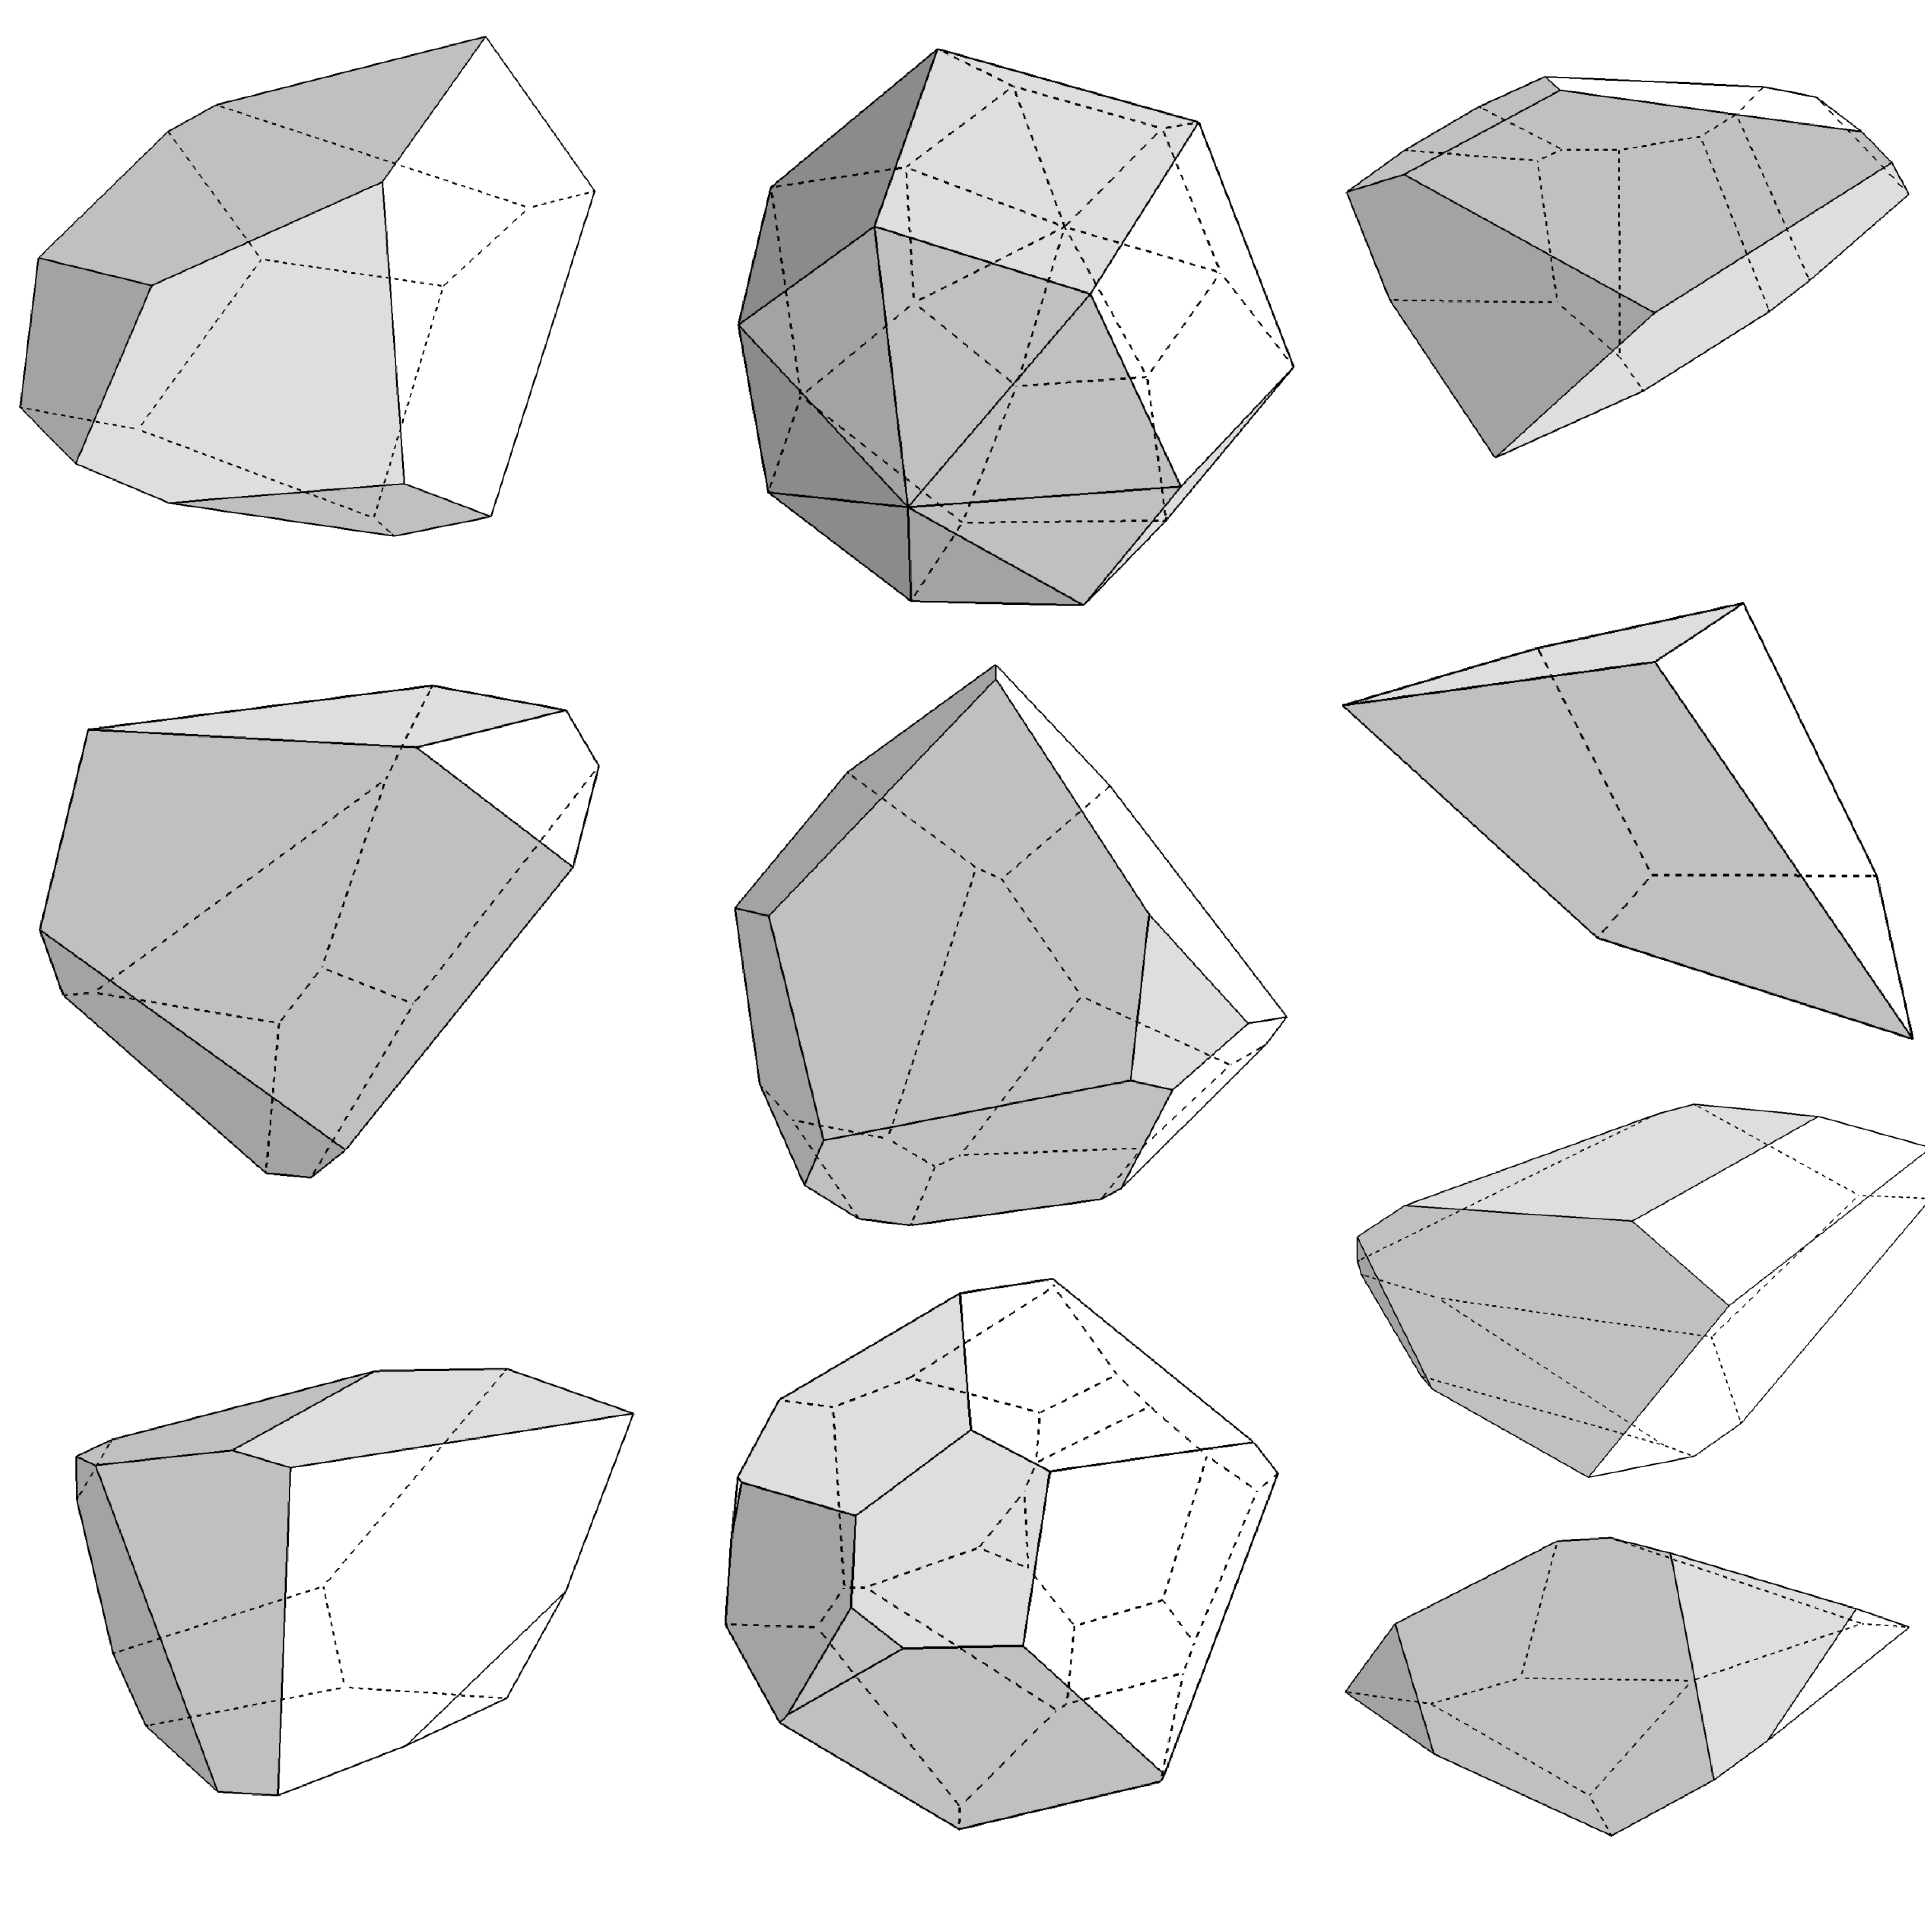
\includegraphics[width=0.5\linewidth]{FV_example.eps}
	\end{figure}

\end{frame}

%SLIDE #?
\begin{frame}{Основные типы сеточных элементов}

	\transdissolve[duration=0.1]
	\justifying
	\large

	Двумерные элементы:

	\begin{center}
		\psset{xunit=1cm,yunit=1cm,algebraic=true}
		\begin{pspicture}(0,0)(7,5)

			\psline[linewidth=1pt, linecolor=black]{*-*}(0,2)(2,4)
			\psline[linewidth=1pt, linecolor=black]{*-*}(2,4)(3,1.5)
			\psline[linewidth=1pt, linecolor=black]{*-*}(3,1.5)(0,2)

			\psline[linewidth=1pt, linecolor=black]{*-*}(4,2)(3,4)
			\psline[linewidth=1pt, linecolor=black]{*-*}(3,4)(5,5)
			\psline[linewidth=1pt, linecolor=black]{*-*}(5,5)(7,3)
			\psline[linewidth=1pt, linecolor=black]{*-*}(7,3)(4,2)

			\uput[0](0,1){Треугольник}
			\uput[0](3.5,1.5){Четырехугольник}

		\end{pspicture}
	\end{center}

\end{frame}

\begin{frame}{Основные типы сеточных элементов}

	\transdissolve[duration=0.1]
	\justifying
	\large

	\begin{center}
		Трёхмерные элементы:
	\end{center}

	\begin{minipage}{0.49\textwidth}
		\begin{center}
			\psset{xunit=1cm,yunit=1cm,algebraic=true}
			\begin{pspicture}(0,0)(7,5)

				\psline[linewidth=1pt, linecolor=black]{*-*}(0,2)(2,4)
				\psline[linewidth=1pt, linecolor=black]{*-*}(2,4)(3,1.5)
				\psline[linewidth=1pt, linecolor=black]{*-*}(2,4)(3,3)
				\psline[linewidth=1pt, linecolor=black]{*-*}(3,3)(3,1.5)
				\psline[linewidth=1pt, linecolor=black]{*-*}(3,1.5)(0,2)
				\psline[linewidth=1pt, linecolor=black, linestyle=dashed](0,2)(3,3)

				\uput[0](0,1){Тетраэдр}

				\psline[linewidth=1pt, linecolor=black]{*-*}(4,1)(3.5,2)
				\psline[linewidth=1pt, linecolor=black, linestyle=dashed](3.5,2)(5,3)
				\psline[linewidth=1pt, linecolor=black, linestyle=dashed](5,3)(7,2)
				\psline[linewidth=1pt, linecolor=black]{*-*}(7,2)(4,1)

				\psline[linewidth=1pt, linecolor=black]{*-*}(4,1)(5,4)
				\psline[linewidth=1pt, linecolor=black]{*-*}(3.5,2)(5,4)
				\psline[linewidth=1pt, linecolor=black, linestyle=dashed](5,3)(5,4)
				\psline[linewidth=1pt, linecolor=black]{*-*}(7,2)(5,4)

				\uput[0](4,0.5){Пирамида}

			\end{pspicture}
		\end{center}
	\end{minipage}
	\hfill
	\begin{minipage}{0.49\textwidth}
		\begin{center}
			\psset{xunit=1cm,yunit=1cm,algebraic=true}
			\begin{pspicture}(0,0)(7,5)

				\psline[linewidth=1pt, linecolor=black]{*-*}(2,5)(3,3.5)
				\psline[linewidth=1pt, linecolor=black]{*-*}(3,3.5)(0,4)
				\psline[linewidth=1pt, linecolor=black]{*-*}(0,4)(2,5)

				\psline[linewidth=1pt, linecolor=black, linestyle=dashed](2,3)(3,1.5)
				\psline[linewidth=1pt, linecolor=black]{*-*}(3,1.5)(0,2)
				\psline[linewidth=1pt, linecolor=black, linestyle=dashed](0,2)(2,3)

				\psline[linewidth=1pt, linecolor=black]{*-*}(0,2)(0,4)
				\psline[linewidth=1pt, linecolor=black]{*-*}(3,1.5)(3,3.5)
				\psline[linewidth=1pt, linecolor=black, linestyle=dashed](2,3)(2,5)

				\uput[0](0,1){Призма}

				\psline[linewidth=1pt, linecolor=black]{*-*}(4,3)(3.5,4)
				\psline[linewidth=1pt, linecolor=black]{*-*}(3.5,4)(5,5)
				\psline[linewidth=1pt, linecolor=black]{*-*}(5,5)(7,4)
				\psline[linewidth=1pt, linecolor=black]{*-*}(7,4)(4,3)

				\psline[linewidth=1pt, linecolor=black]{*-*}(4,3)(4,1)
				\psline[linewidth=1pt, linecolor=black]{*-*}(3.5,4)(3.5,2)
				\psline[linewidth=1pt, linecolor=black, linestyle=dashed](5,5)(5,3)
				\psline[linewidth=1pt, linecolor=black]{*-*}(7,4)(7,2)

				\psline[linewidth=1pt, linecolor=black]{*-*}(4,1)(3.5,2)
				\psline[linewidth=1pt, linecolor=black, linestyle=dashed](3.5,2)(5,3)
				\psline[linewidth=1pt, linecolor=black, linestyle=dashed](5,3)(7,2)
				\psline[linewidth=1pt, linecolor=black]{*-*}(7,2)(4,1)

				\uput[0](4,0.5){Шестигранник}

			\end{pspicture}
		\end{center}
	\end{minipage}

\end{frame}

%SLIDE #?
\begin{frame}{Обшая классификация сеток}

	\transdissolve[duration=0.1]
	\justifying
	\large

	\begin{center}
		\tikzstyle{root concept}+=[concept color=blue!80,minimum size=3.5cm]
		\tikz[mindmap]
			\node [concept] {Основные типы сеток}
				child[concept color=yellow, grow=24, minimum size=3cm]
				{
					node[concept](root1) at (0,0) {Структу-\\рированные (регулярные) сетки}
				}
				child[concept color=green, grow=0, minimum size=3cm]
				{
					node[concept](root2) at (2,0) {Блочно -- структу-\\рированные сетки}
				}
				child[concept color=red, grow=-24, minimum size=3cm]
				{
					node[concept](root2) at (0,0) {Неструкту-\\рированные сетки}
				};
	\end{center}

\end{frame}

%SLIDE #?
\begin{frame}{Структурированные сетки}

	\transdissolve[duration=0.1]
	\justifying
	\large

	\begin{center}
		\tikzstyle{root concept}+=[concept color=blue!80,minimum size=3.5cm]
		\tikz[mindmap]
			\node [concept] {Структу-\\рированные (регулярные) сетки}
				child[concept color=yellow, grow=24, minimum size=3cm]
				{
					node[concept](root1) at (0,0) {Орто-\\гональные}
				}
				child[concept color=green, grow=0, minimum size=3cm]
				{
					node[concept](root2) at (2,0) {Неорто-\\гональные}
				}
				child[concept color=red, grow=-24, minimum size=3cm]
				{
					node[concept](root2) at (0,0) {H - типа, O - типа, C - типа, L - типа, Y - типа}
				};
	\end{center}

\end{frame}

%SLIDE #?
\begin{frame}{Свойства регулярных сеток}

	\transdissolve[duration=0.1]
	\justifying
	\large

	\begin{itemize}
		\justifying
		\item Структурированные (регулярные) состоят из \textbf{семейств линий}, таких что члены одного семейства \textbf{не пересекаются} между собой и \textbf{пересекают} любую линию из другого семейства \textbf{только один раз}.
		\item В структурированных сетках \textbf{положение любой точки} сетки (или контрольного объема) в области уникально \textbf{определяется набором двух} (в $2D$) \textbf{или трех} (в $3D$) индексов, например, $(i, j, k)$.
		\item Логически эквивалетна декартовой сетке.
	\end{itemize}

\end{frame}

%SLIDE #?
\begin{frame}{Достоинства регулярных сеток}

	\transdissolve[duration=0.1]
	\justifying
	\large

	\begin{itemize}
		\justifying
		\item[+] \textbf{Простота описания}: один из индексов каждой соседней точки $P$ отличается на 1 от соответствующего индекса точки $P$.
		\item[+] При дискретизации уравнений в ч. п. результирующая \textbf{матрица системы алгербраических уравнений} обладает \textbf{регулярной структурой}, что может использовано при разработке метода решения.
	\end{itemize}

\end{frame}

%SLIDE #?
\begin{frame}{Недостатки регулярных сеток}

	\transdissolve[duration=0.1]
	\justifying
	\large

	\begin{itemize}
		\justifying
		\item[-] Применение только в простых геометриях расчетной области.
		\item[-] Измельчение сетки в одной области влечет слишком мелкую сетку в других областях решения и бесполезную трату ресурсов. Длинные узкие ячейки могут плохо влиять на сходимость.
	\end{itemize}

\end{frame}

%SLIDE #?
\begin{frame}{Пример структурированной сетки}

	\transdissolve[duration=0.1]
	\justifying
	\large

	\begin{figure}
		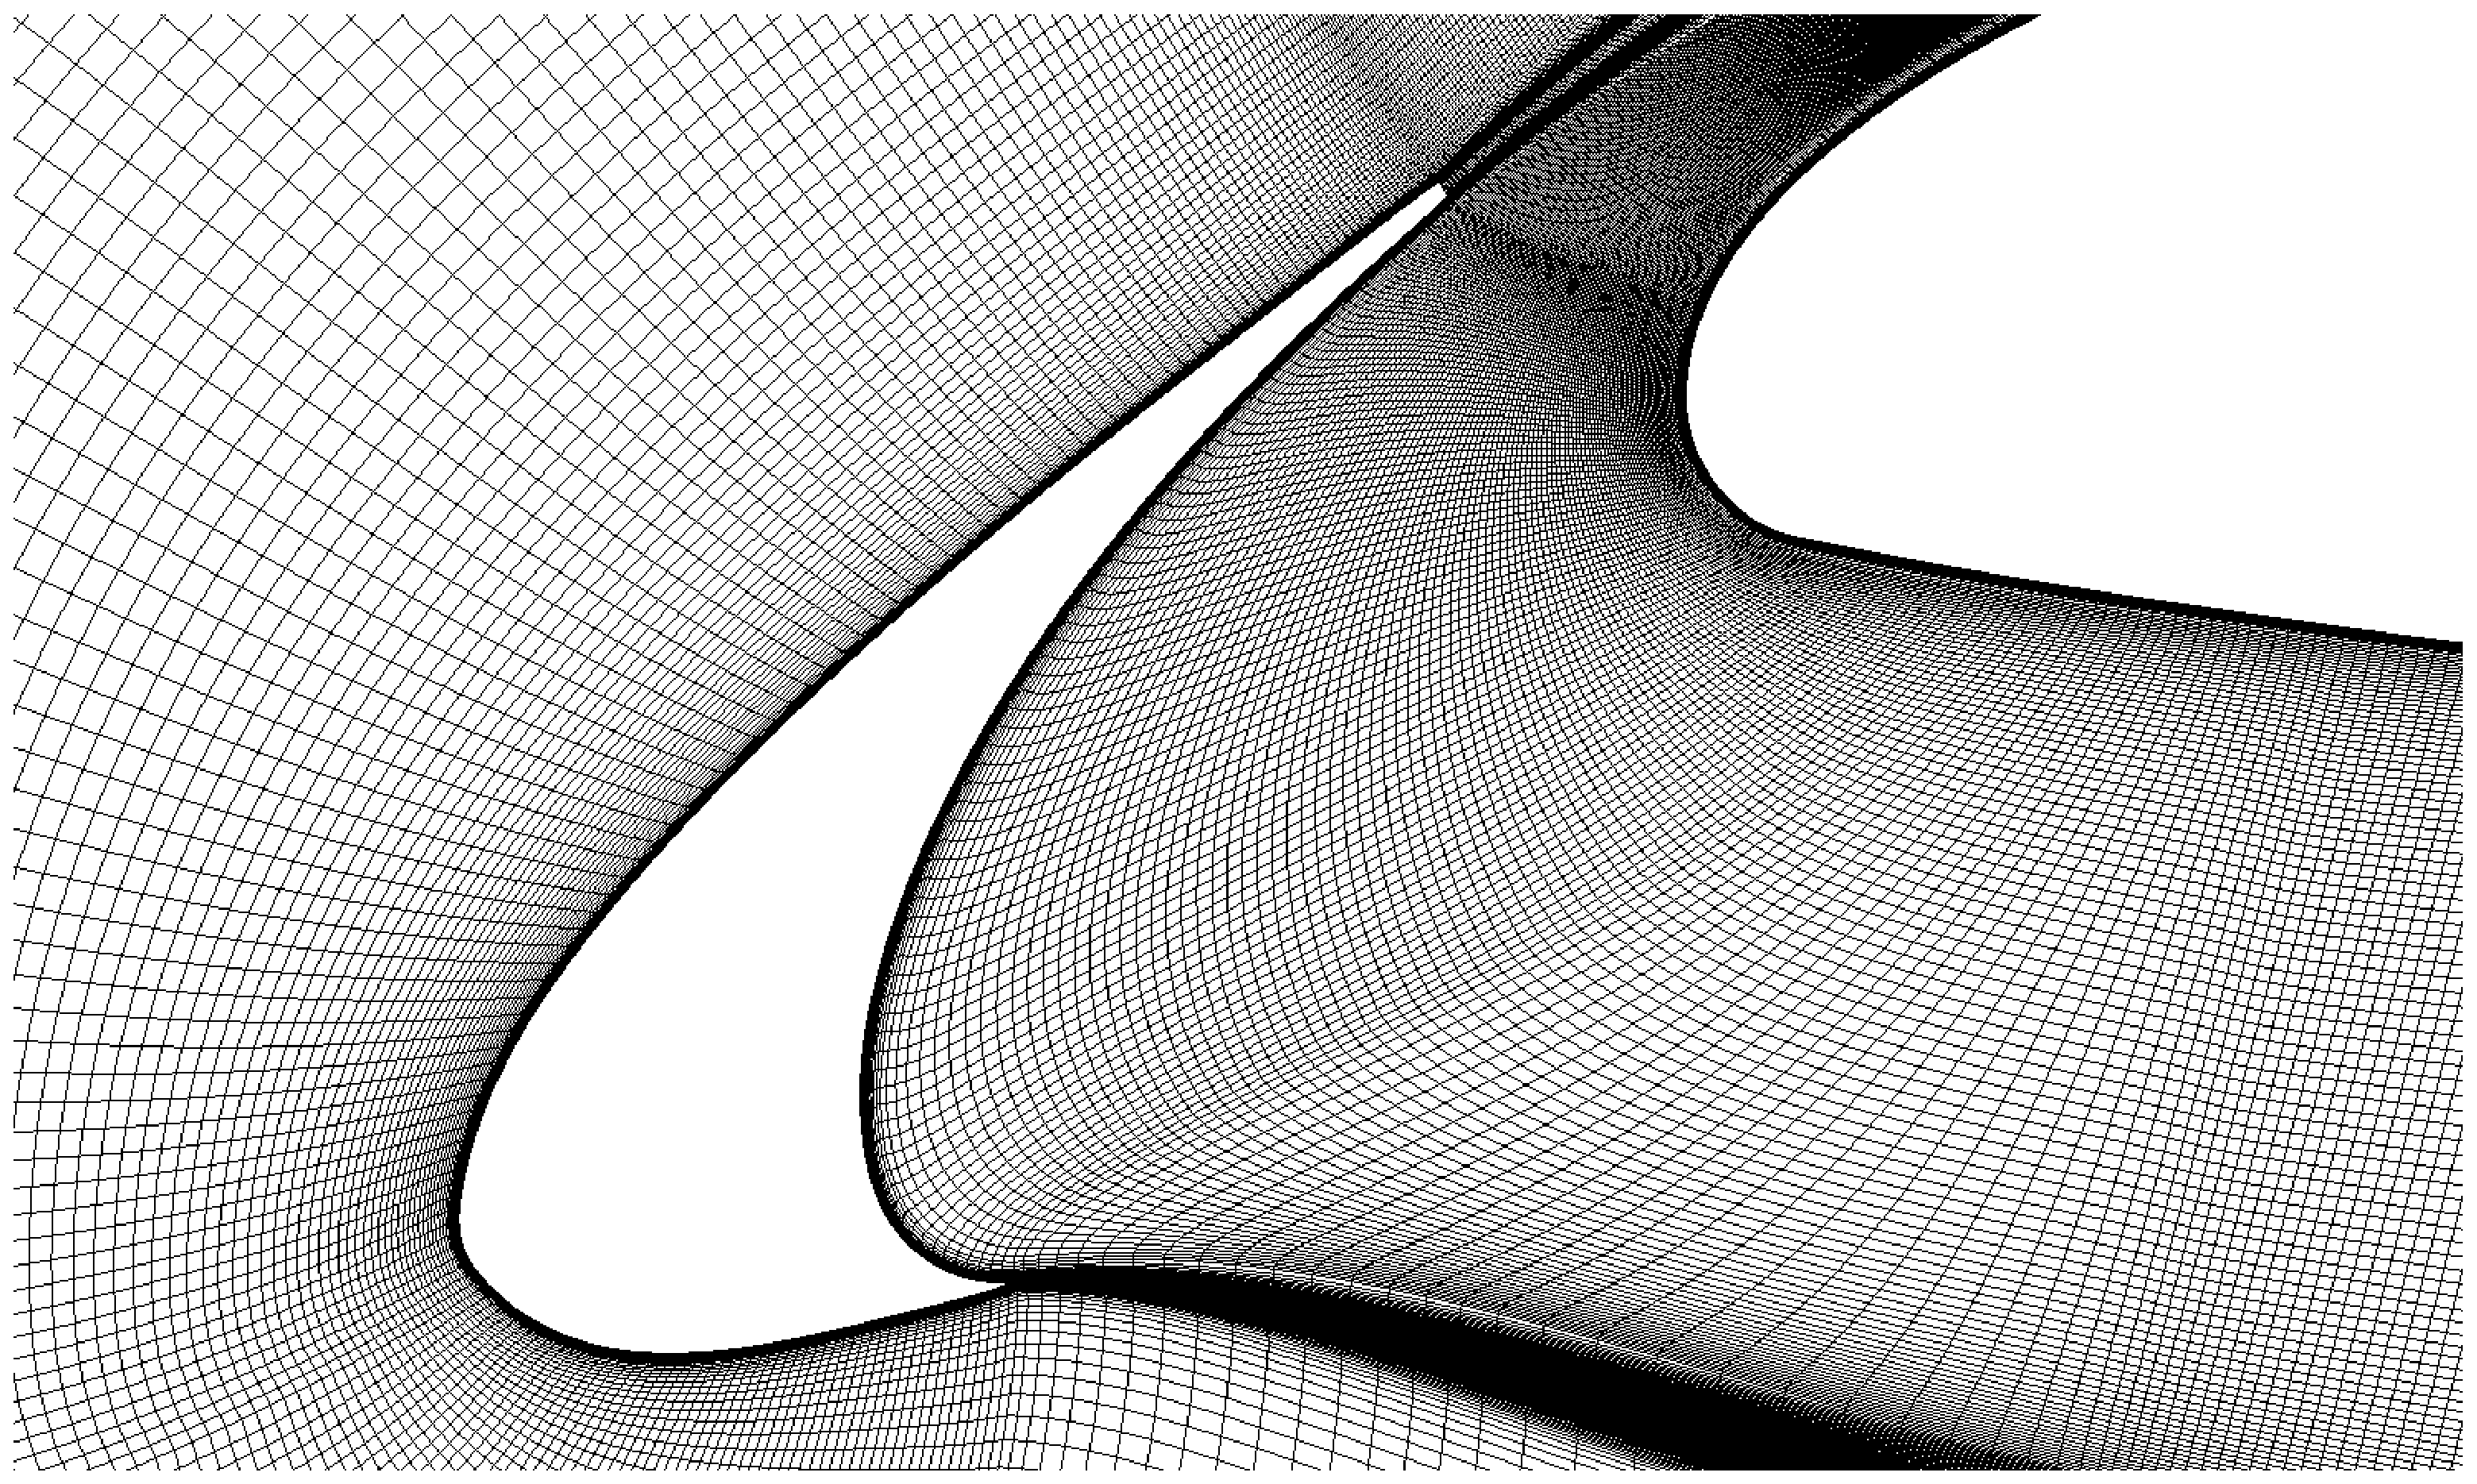
\includegraphics[width=0.8\linewidth]{structured_grid_example.eps}
	\end{figure}

\end{frame}

%SLIDE #?
\begin{frame}{Cетка H - типа}

	\transdissolve[duration=0.1]
	\justifying
	\large

	\begin{figure}
		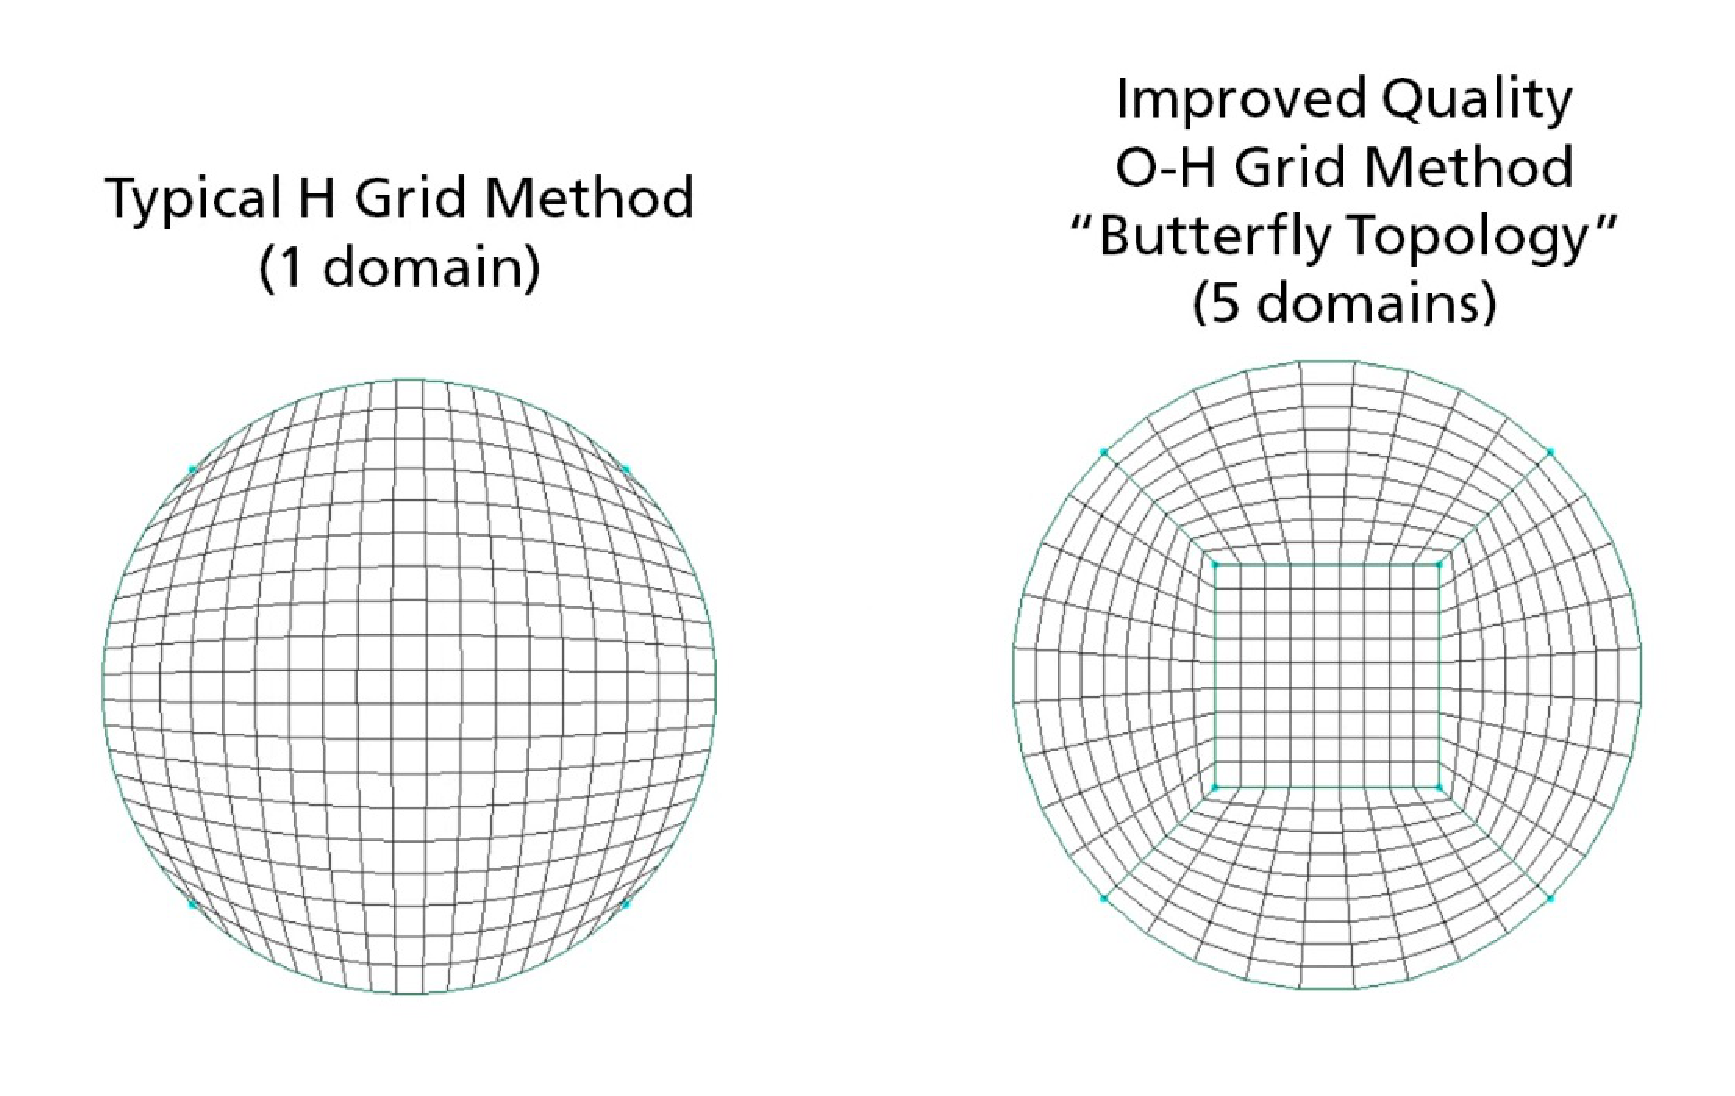
\includegraphics[width=0.8\linewidth]{H_type_grid_example.eps}
	\end{figure}

\end{frame}

%SLIDE #?
\begin{frame}{Cетка O - типа}

	\transdissolve[duration=0.1]
	\justifying
	\large

	\begin{figure}
		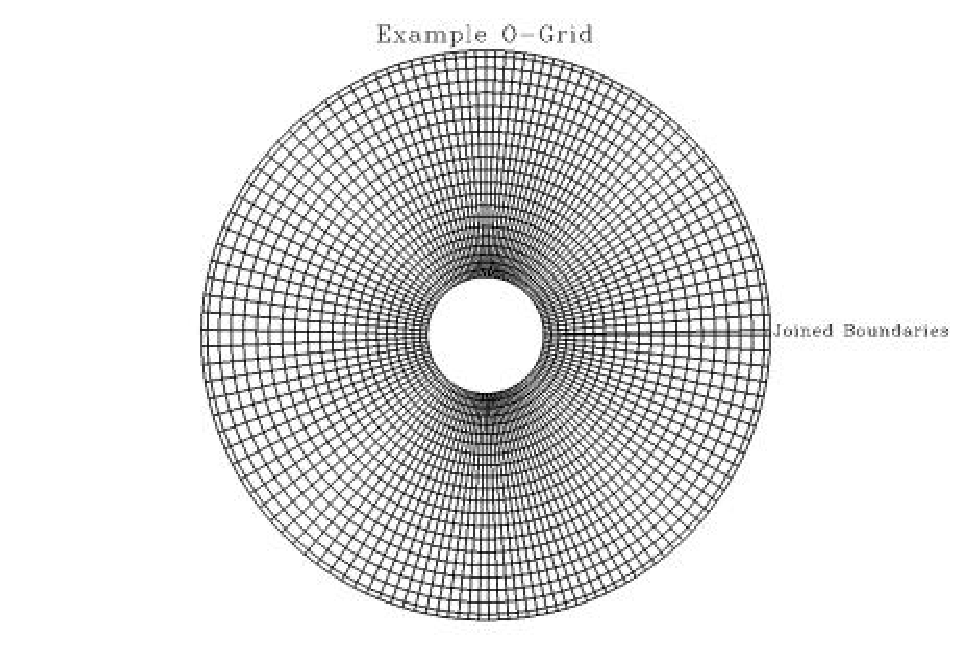
\includegraphics[width=0.7\linewidth]{O_type_grid_example_1.eps}
	\end{figure}

\end{frame}

%SLIDE #?
\begin{frame}{Cетка O - типа}

	\transdissolve[duration=0.1]
	\justifying
	\large

	\begin{figure}
		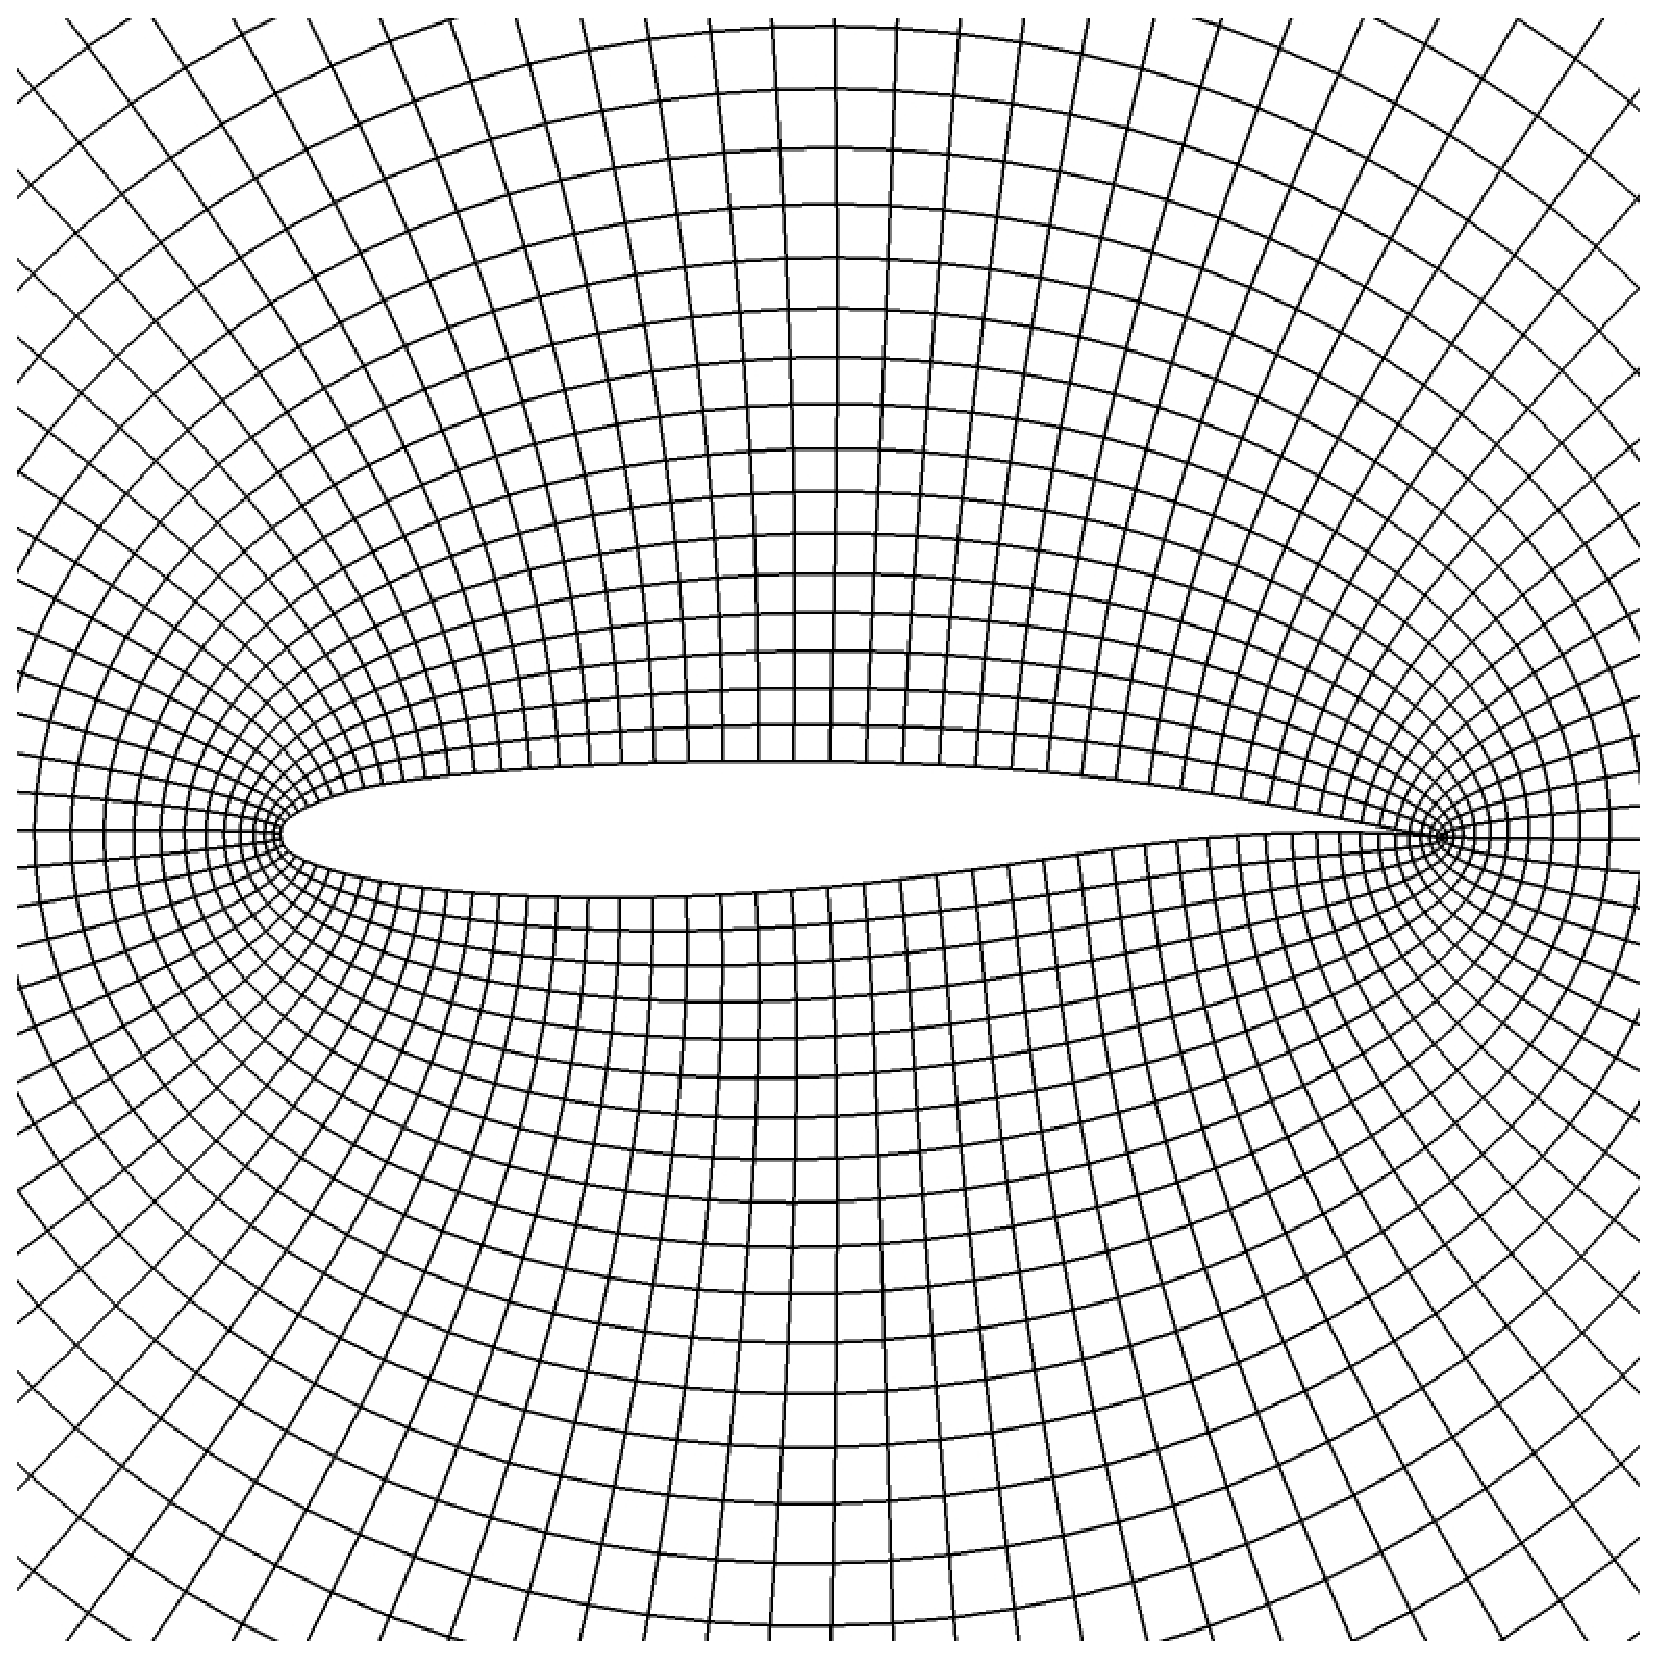
\includegraphics[width=0.5\linewidth]{O_type_grid_example_2.eps}
	\end{figure}

\end{frame}

%SLIDE #?
\begin{frame}{Cетка C - типа}

	\transdissolve[duration=0.1]
	\justifying
	\large

	\begin{figure}
		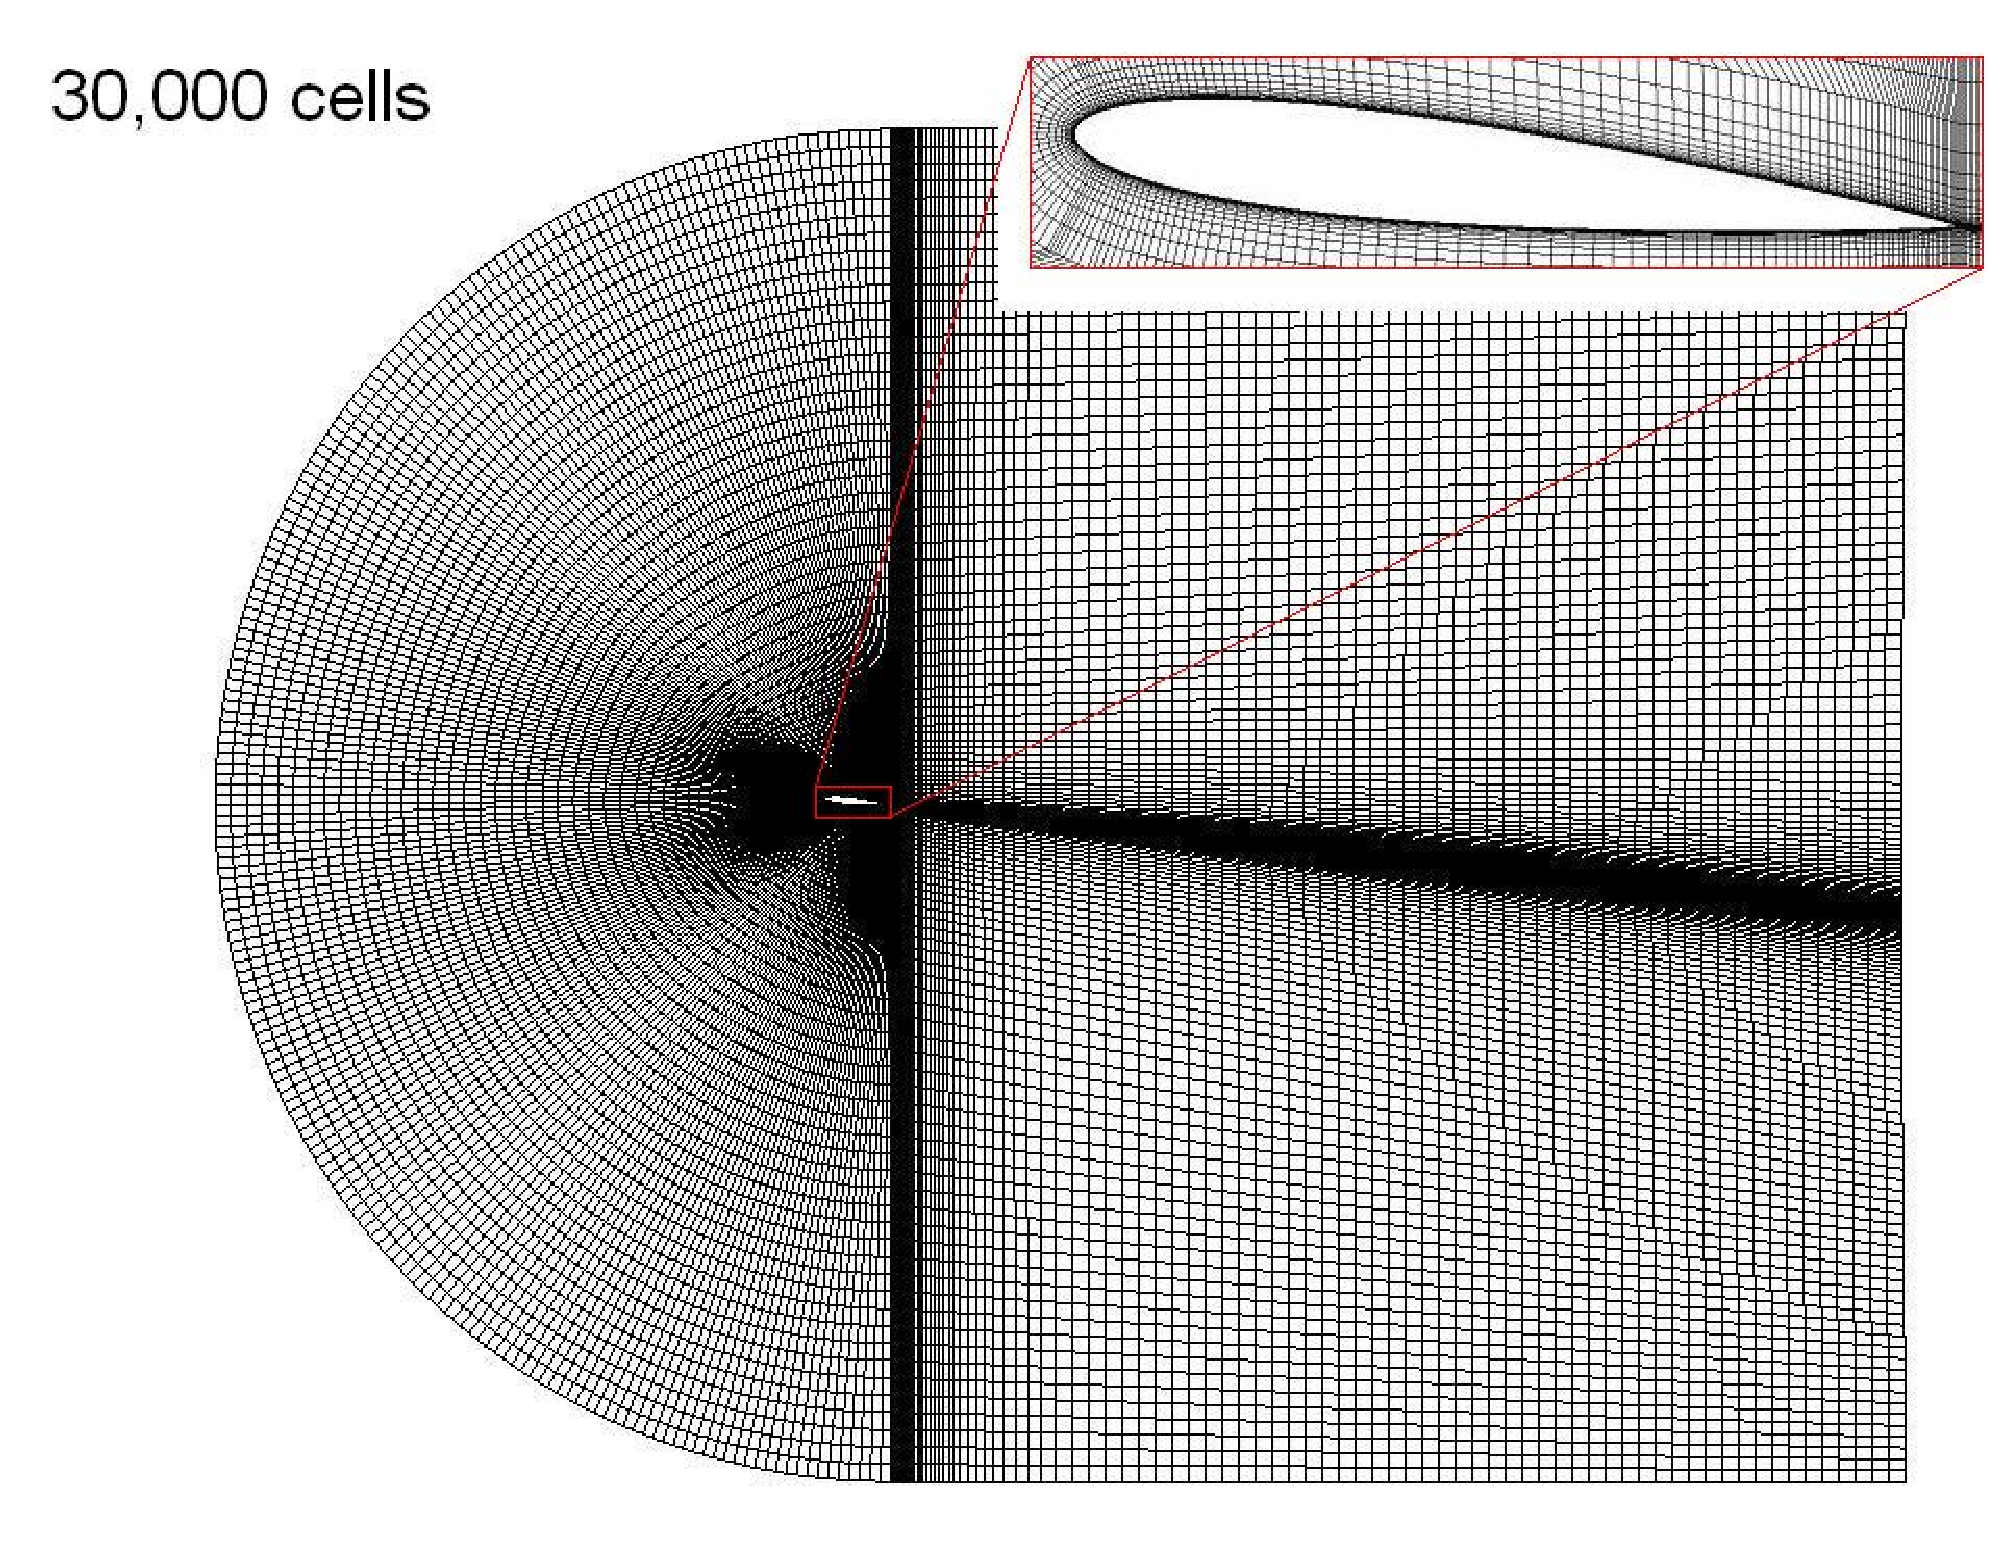
\includegraphics[width=0.6\linewidth]{C_type_grid_example.eps}
	\end{figure}

\end{frame}

%SLIDE #?
\begin{frame}{Cетка C - типа}

	\transdissolve[duration=0.1]
	\justifying
	\large

	\begin{minipage}{0.49\textwidth}
		\begin{center}
			\begin{figure}
				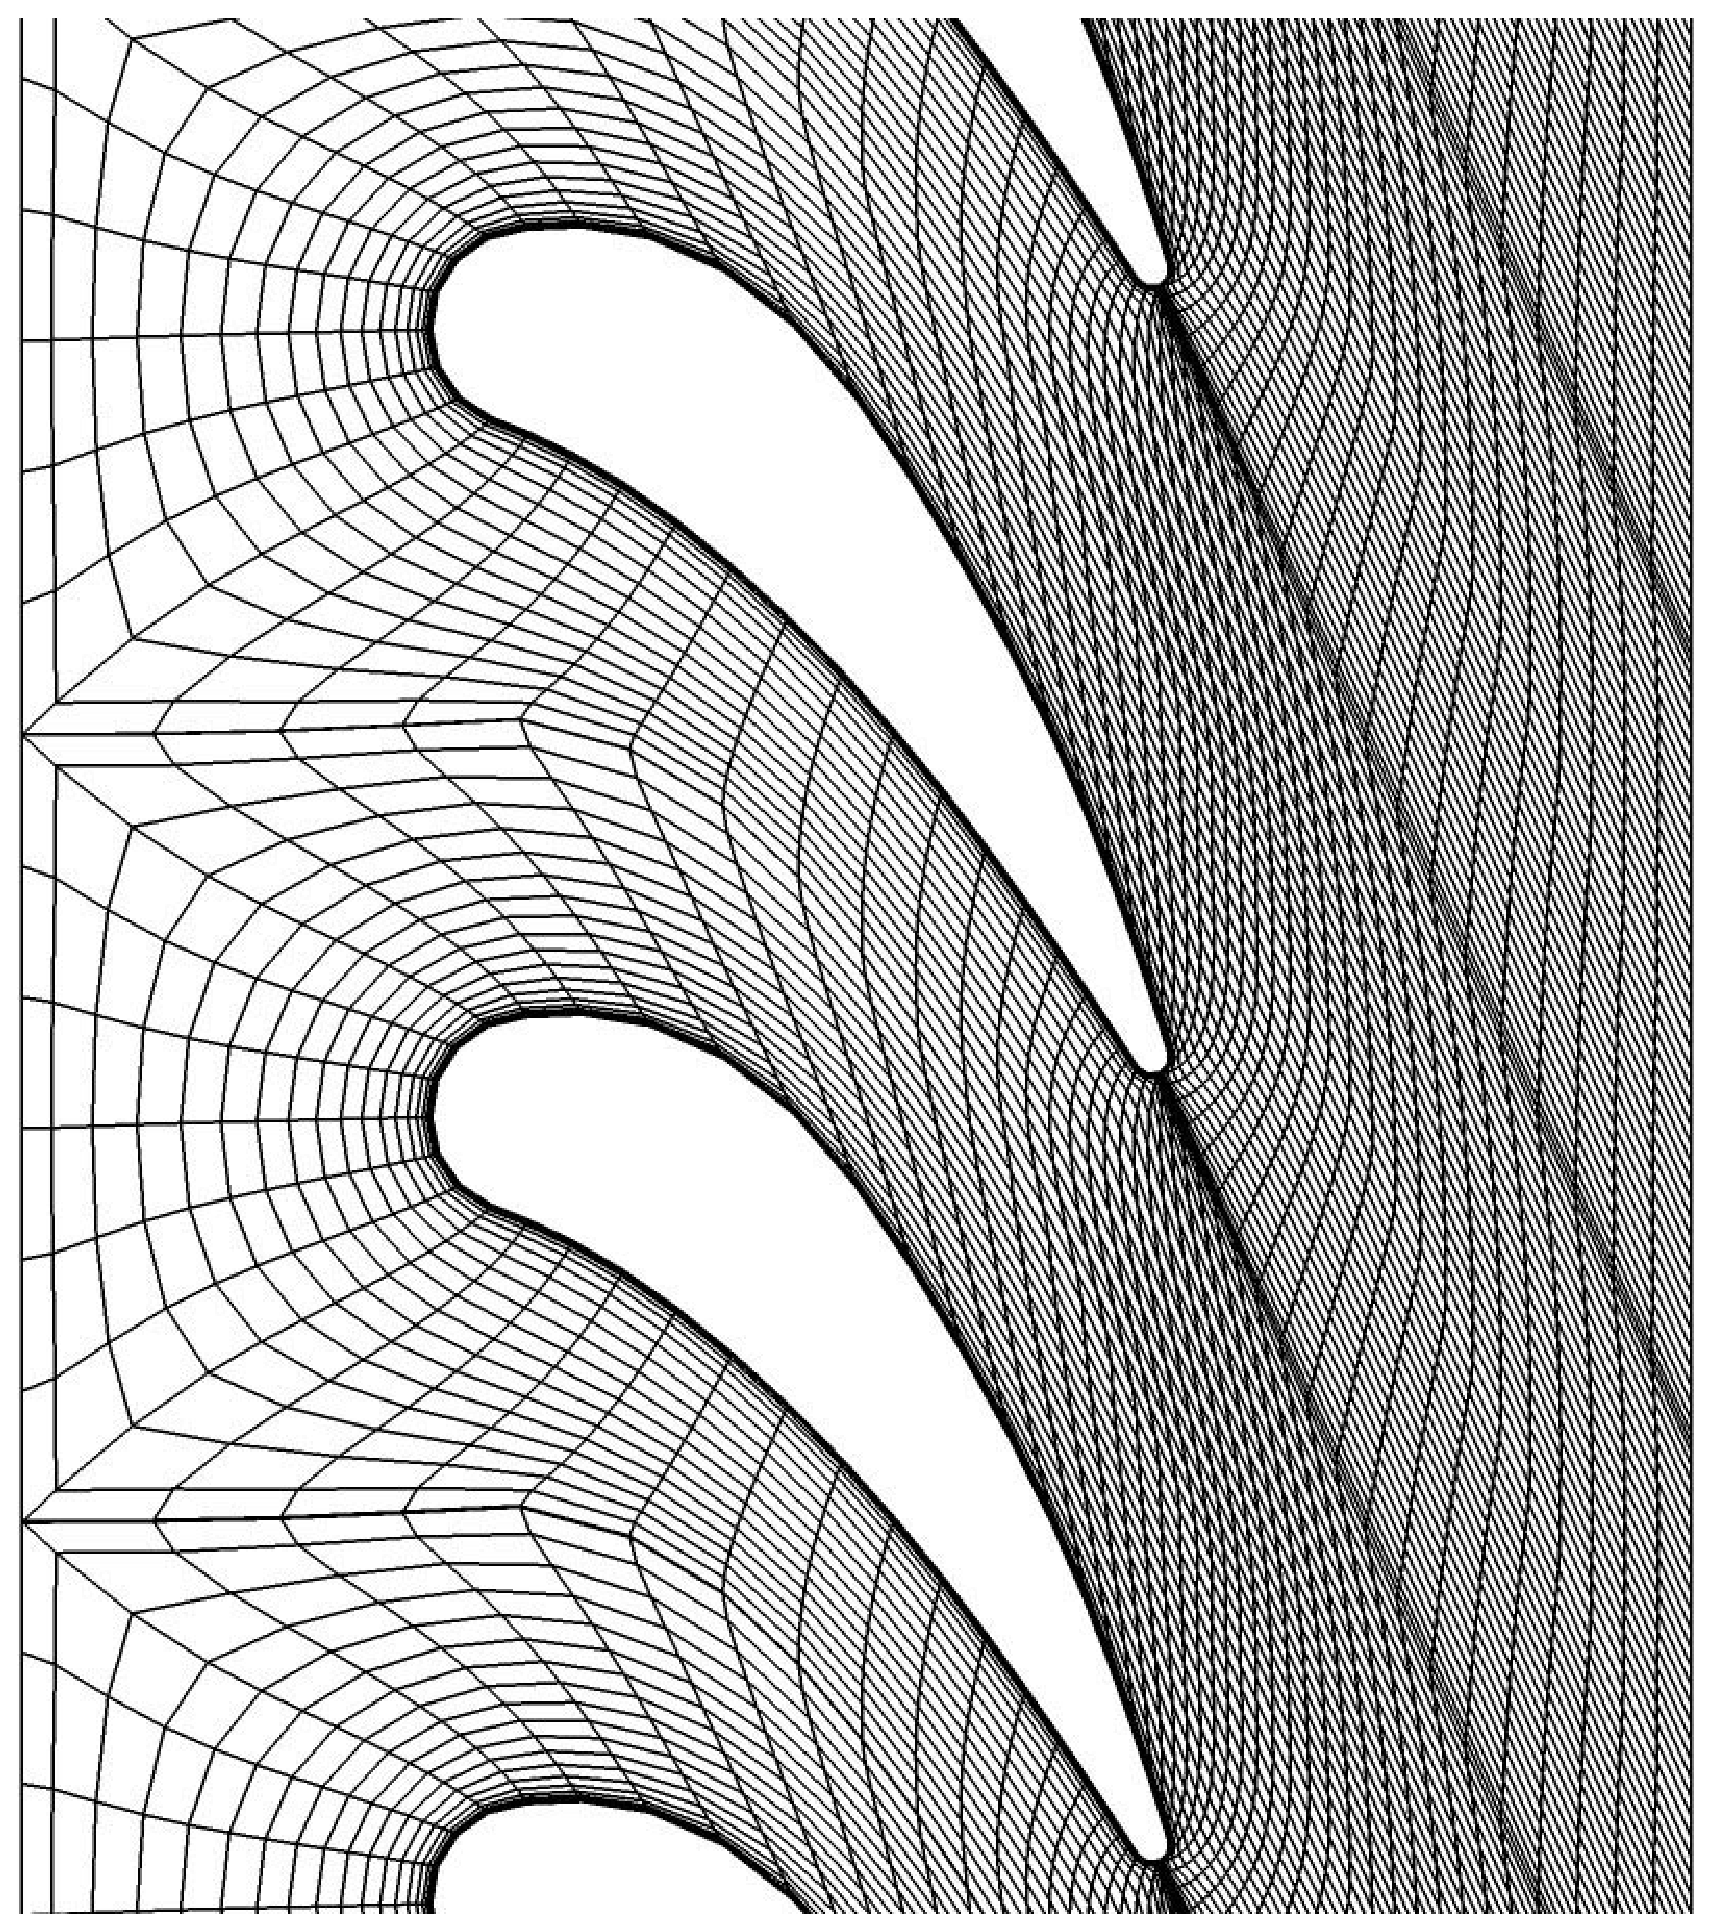
\includegraphics[width=0.8\linewidth]{C_type_grid_example_2.eps}
			\end{figure}
		\end{center}
	\end{minipage}
	\hfill
	\begin{minipage}{0.49\textwidth}
		\begin{center}
			\begin{figure}
				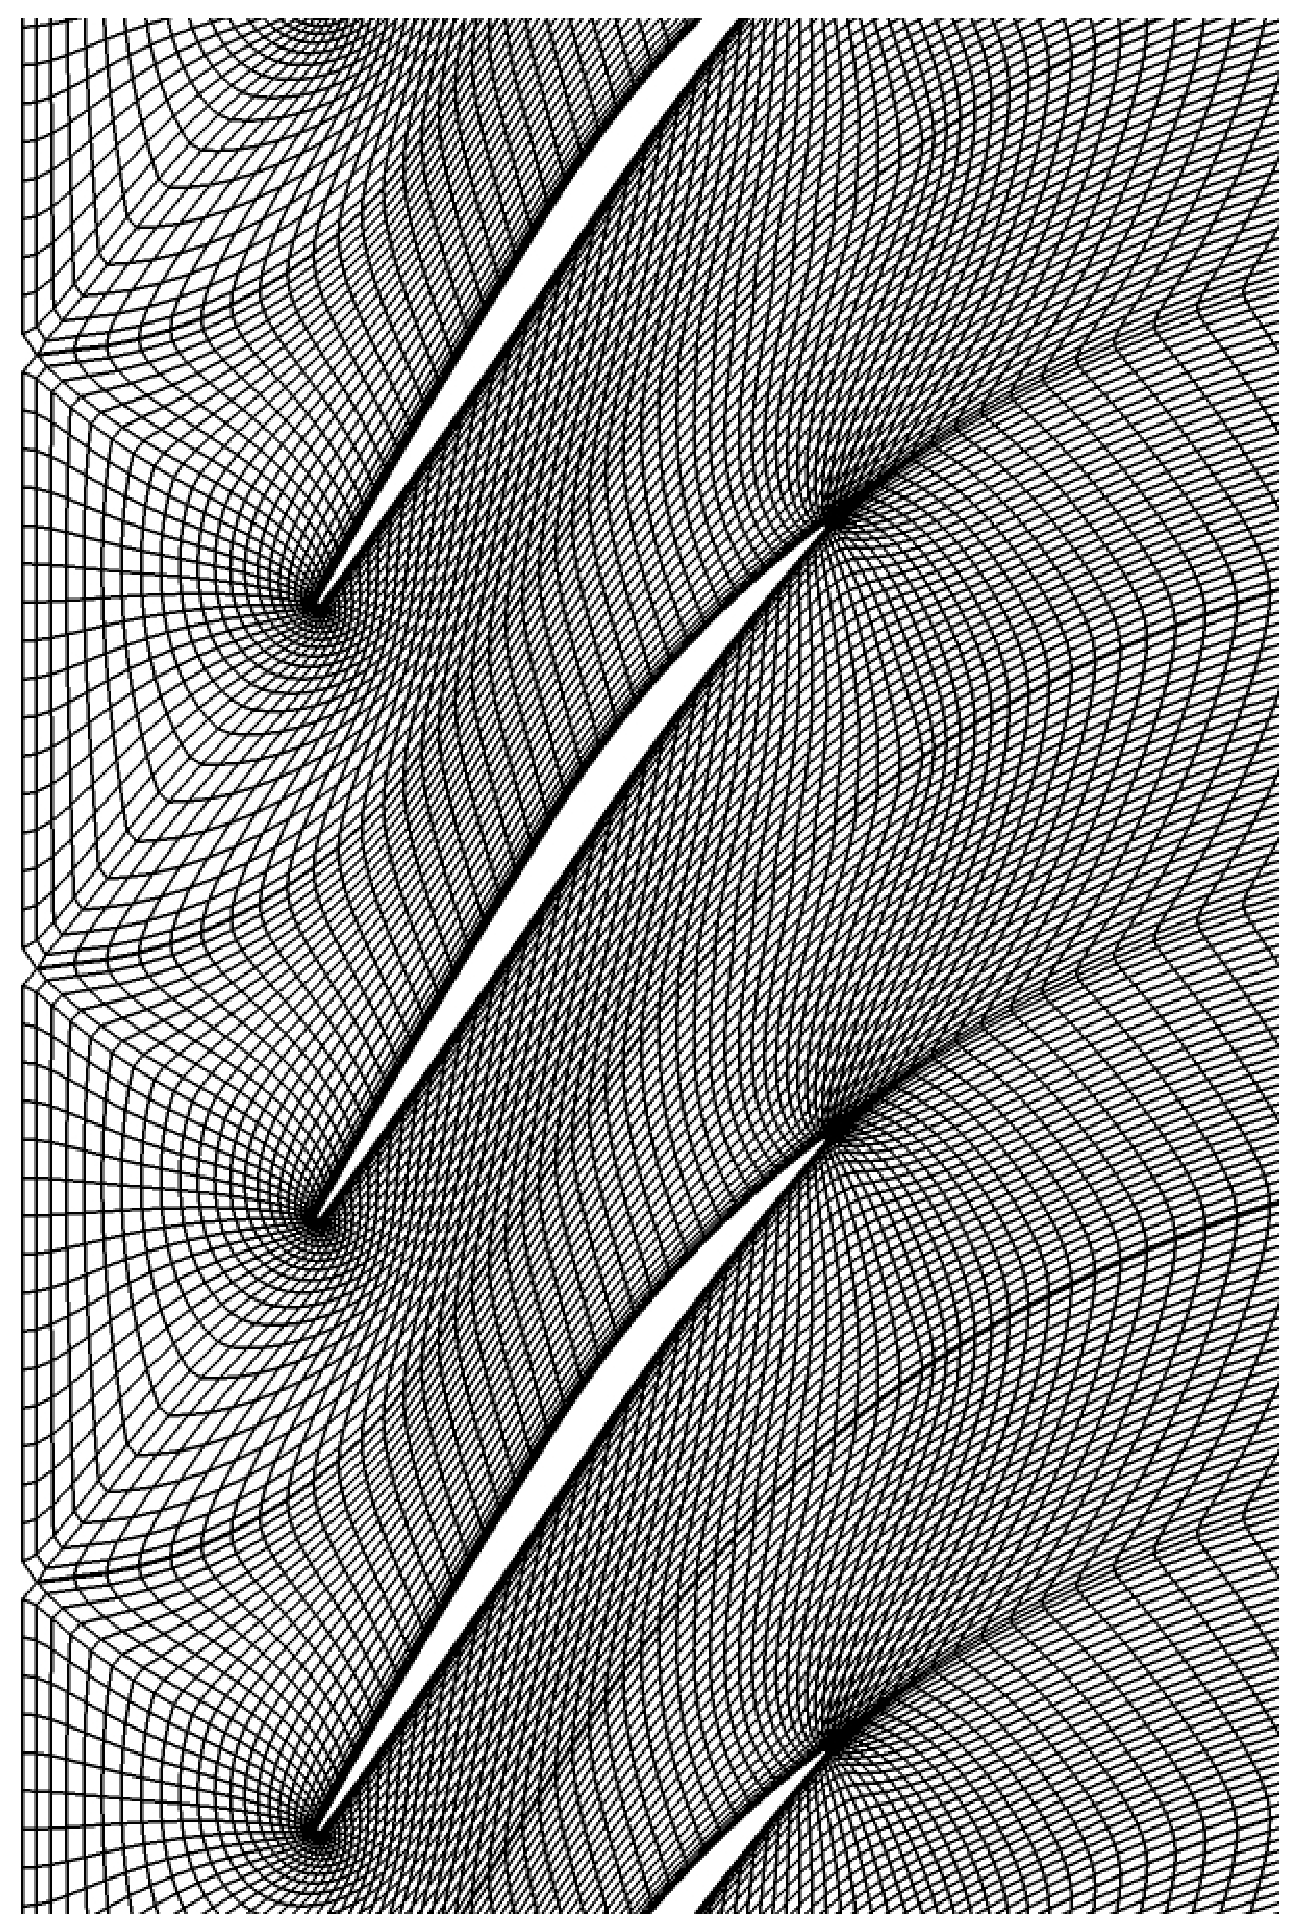
\includegraphics[width=0.6\linewidth]{C_type_grid_example_4.eps}
			\end{figure}
		\end{center}
	\end{minipage}

\end{frame}
%SLIDE #?
\begin{frame}{Cетка C - типа}

	\transdissolve[duration=0.1]
	\justifying
	\large

	\begin{figure}
		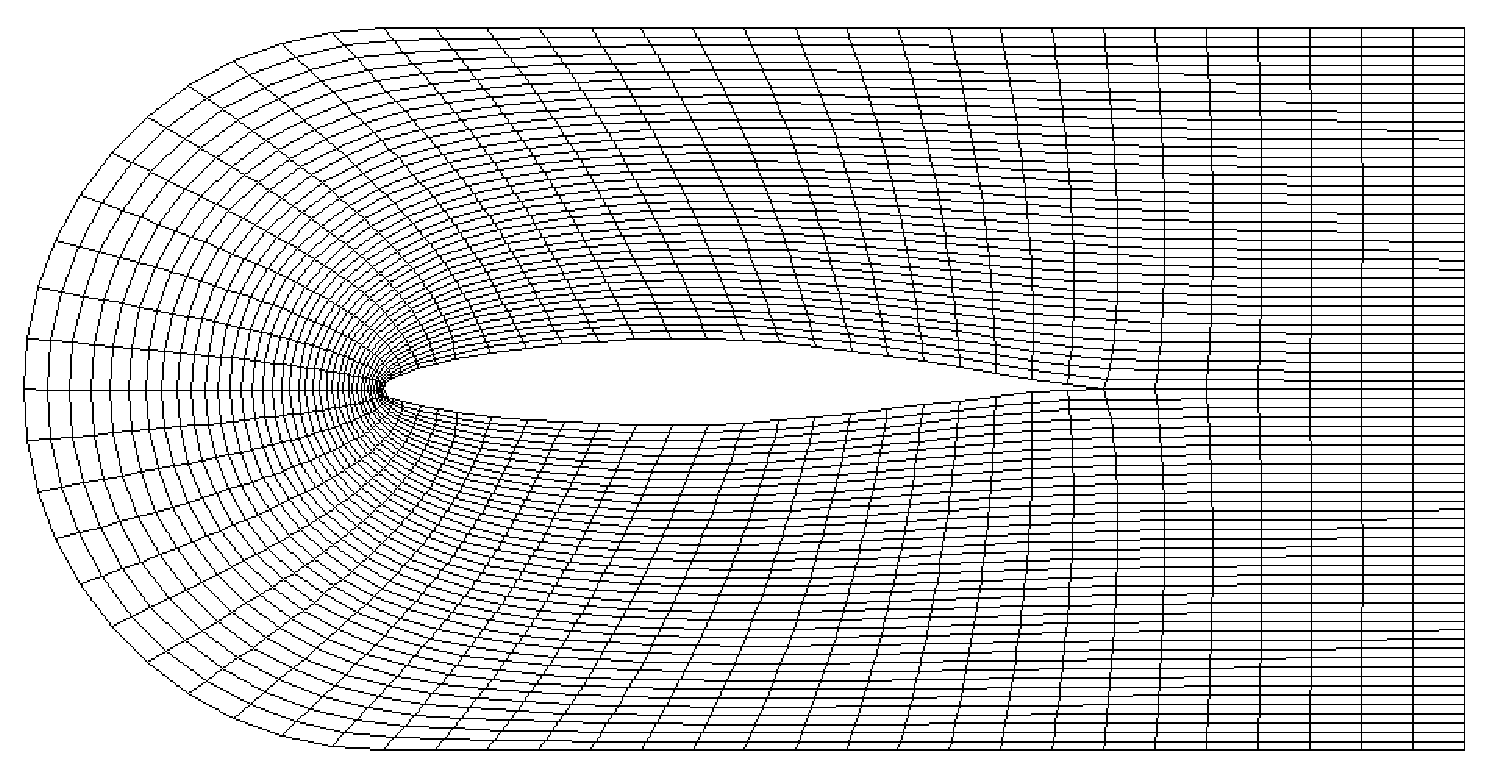
\includegraphics[width=0.8\linewidth]{C_type_grid_example_3.eps}
	\end{figure}

\end{frame}

%SLIDE #?
\begin{frame}{Cетка C - типа}

	\transdissolve[duration=0.1]
	\justifying
	\large

	\begin{figure}
		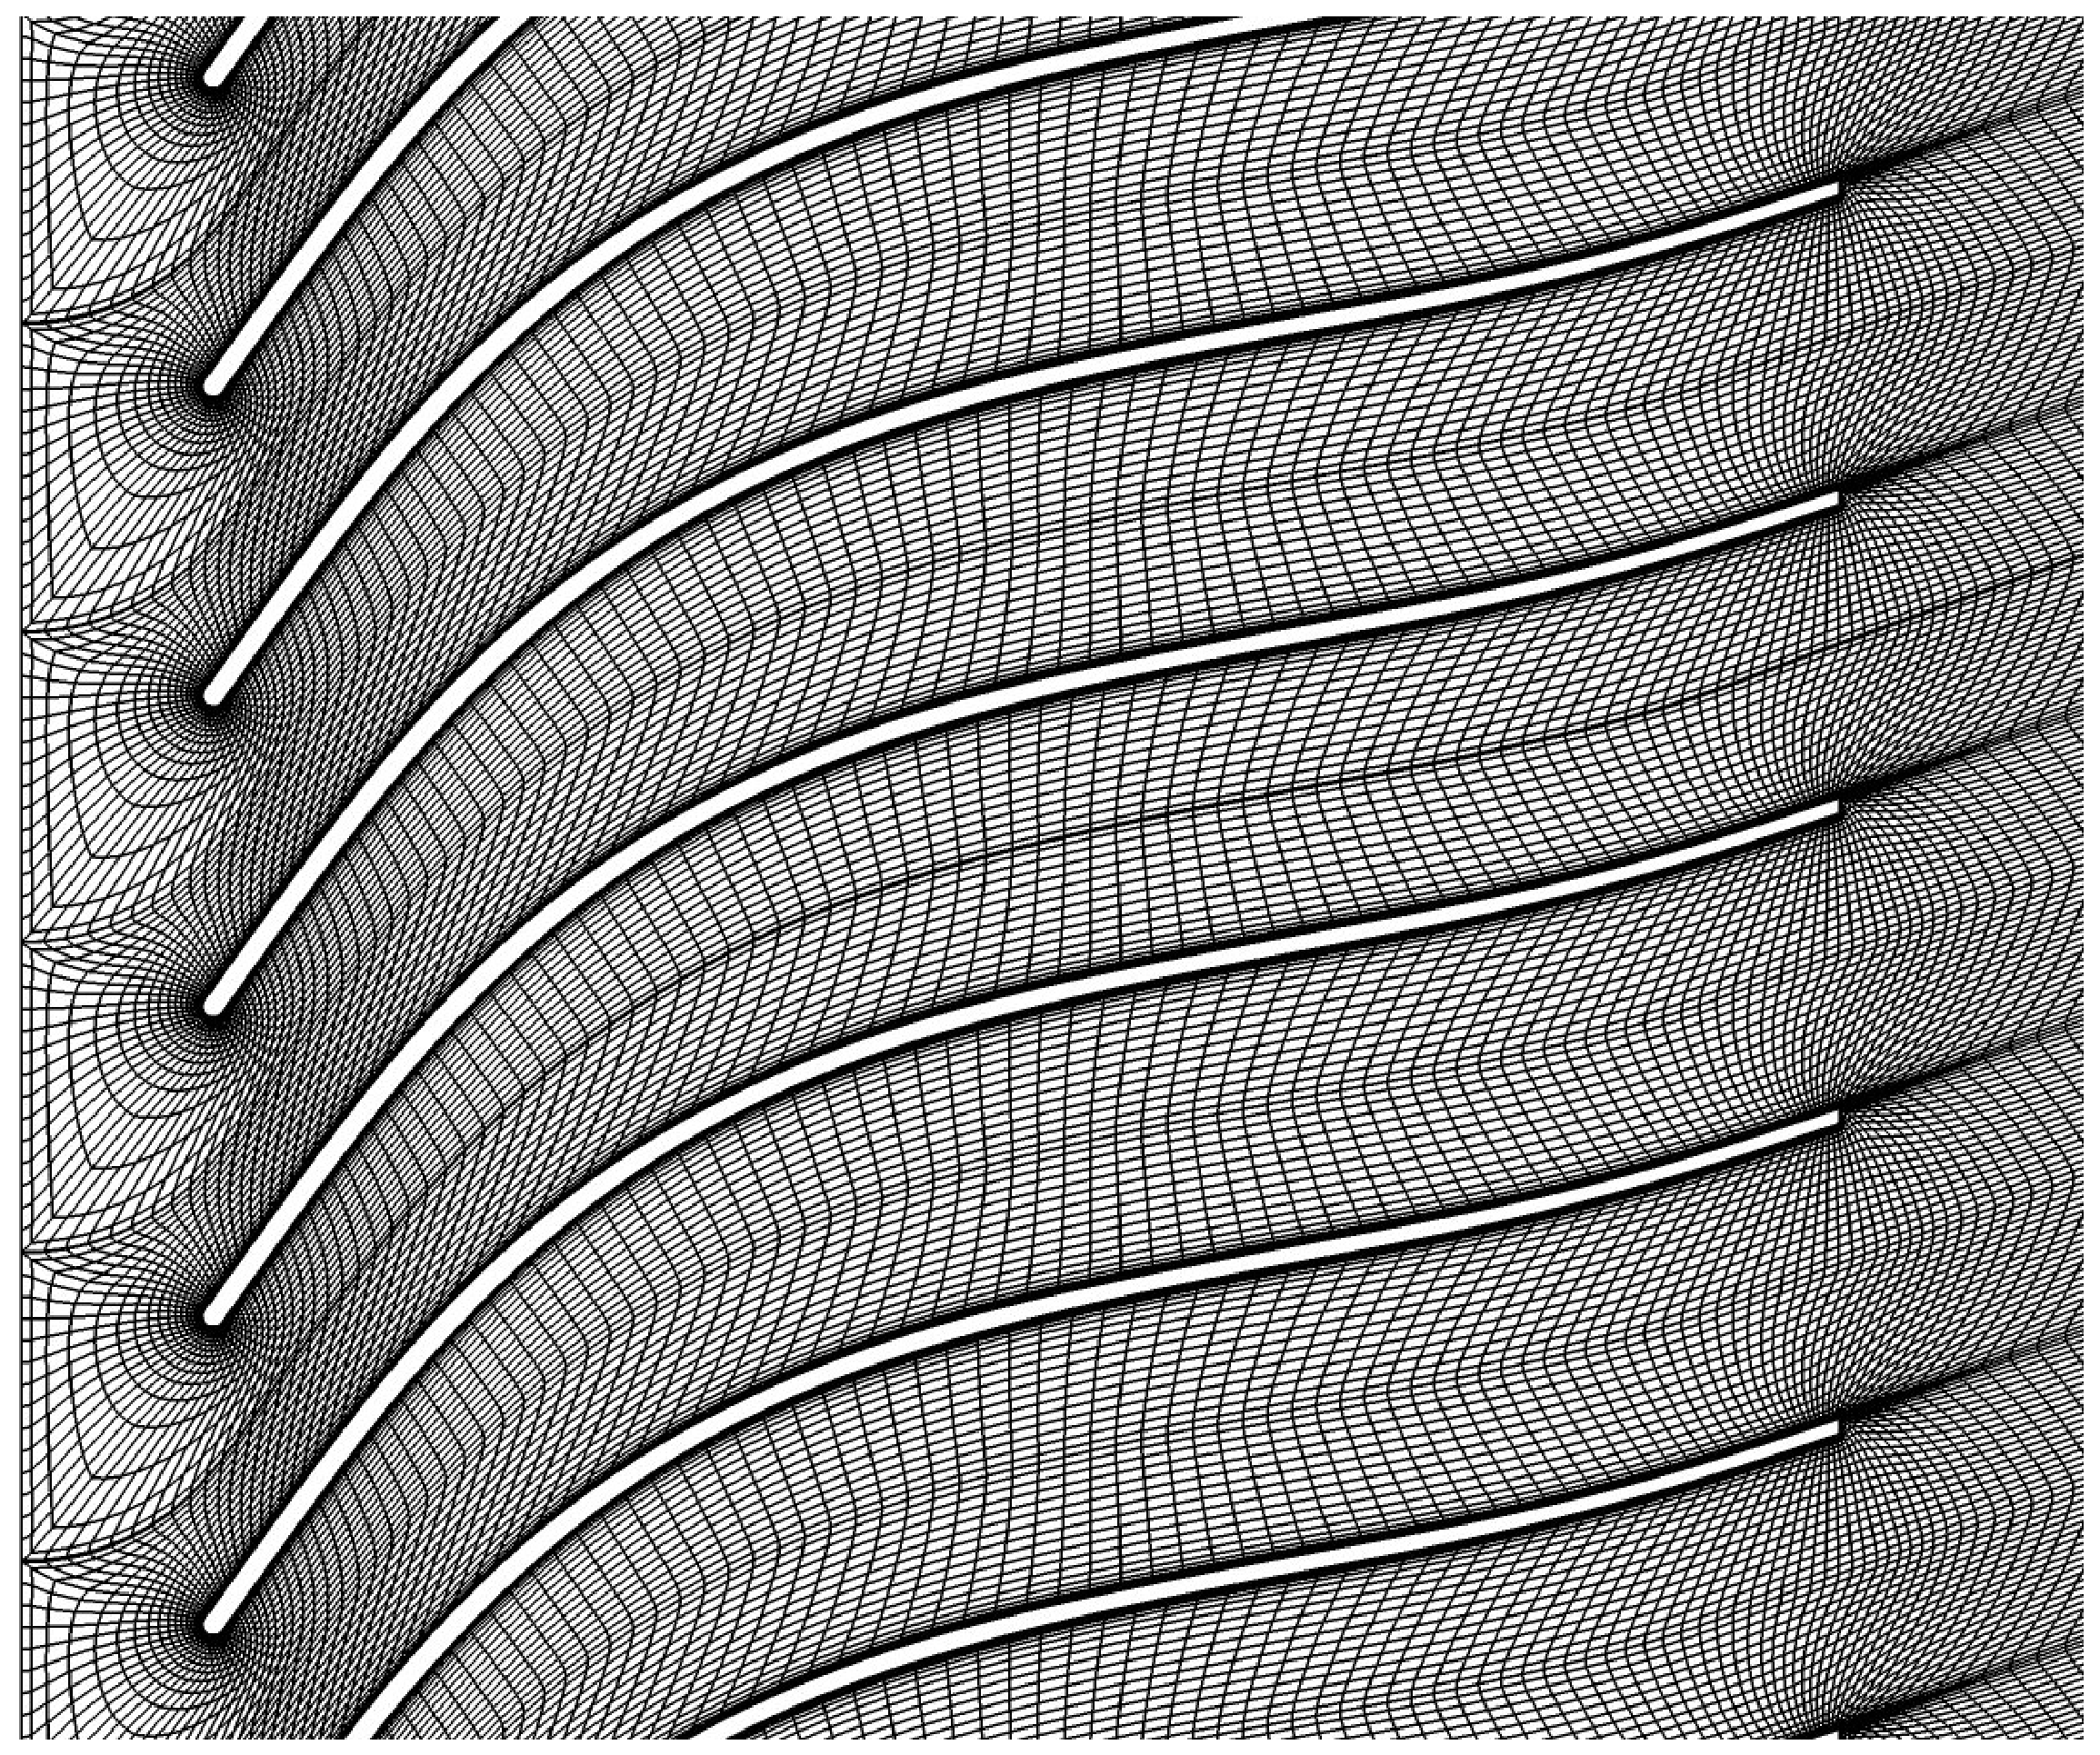
\includegraphics[width=0.55\linewidth]{C_type_grid_example_5.eps}
	\end{figure}

\end{frame}

%SLIDE #?
\begin{frame}{Как построить структурированную сетку для треугольника?}

	\transdissolve[duration=0.1]
	\justifying
	\large

	\begin{center}
		\psset{xunit=1cm,yunit=1cm,algebraic=true}
		\begin{pspicture}(0,0)(6,4)

			\psline[linewidth=2pt, linecolor=black]{*-*}(0,0)(6,0)
			\psline[linewidth=2pt, linecolor=black]{*-*}(6,0)(3,4)
			\psline[linewidth=2pt, linecolor=black]{*-*}(3,4)(0,0)

		\end{pspicture}
	\end{center}

\end{frame}

%SLIDE #?
\begin{frame}{Cетка Y - типа}

	\transdissolve[duration=0.1]
	\justifying
	\large

	\begin{figure}
		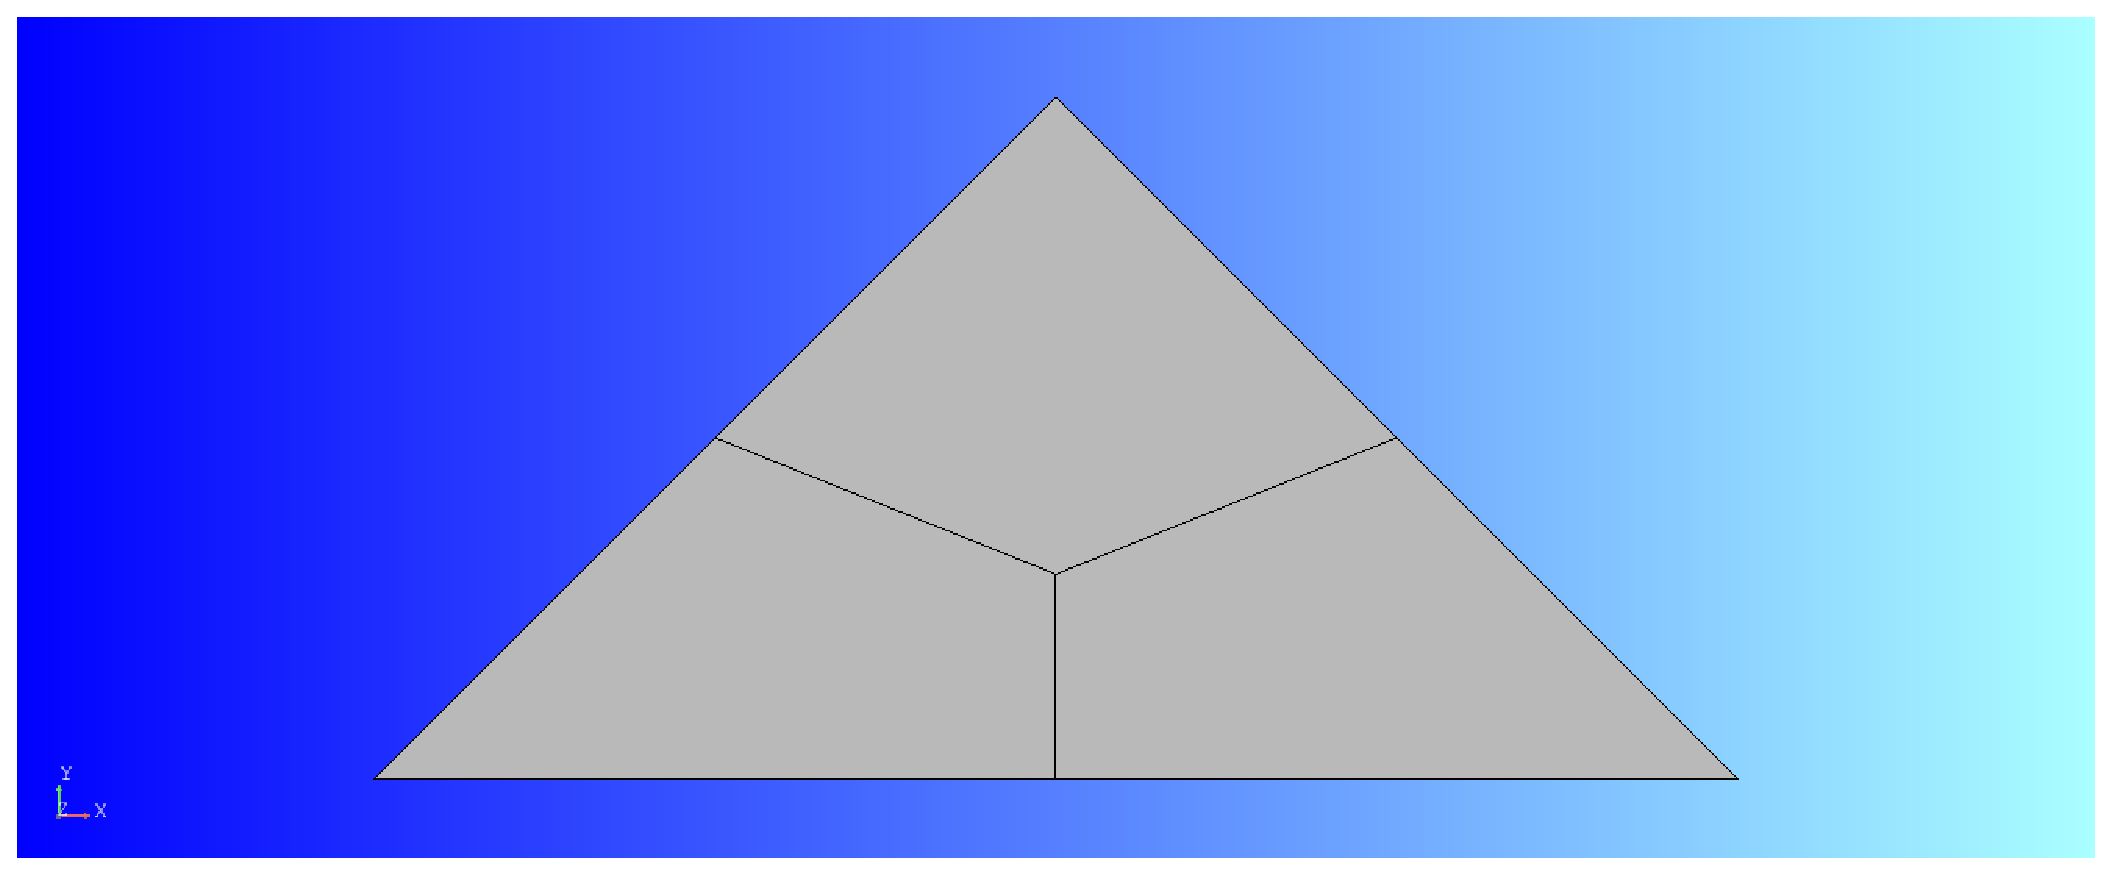
\includegraphics[width=1\linewidth]{triangle_geometry.eps}
	\end{figure}

\end{frame}

%SLIDE #?
\begin{frame}{Cетка Y - типа}

	\transdissolve[duration=0.1]
	\justifying
	\large

	\begin{figure}
		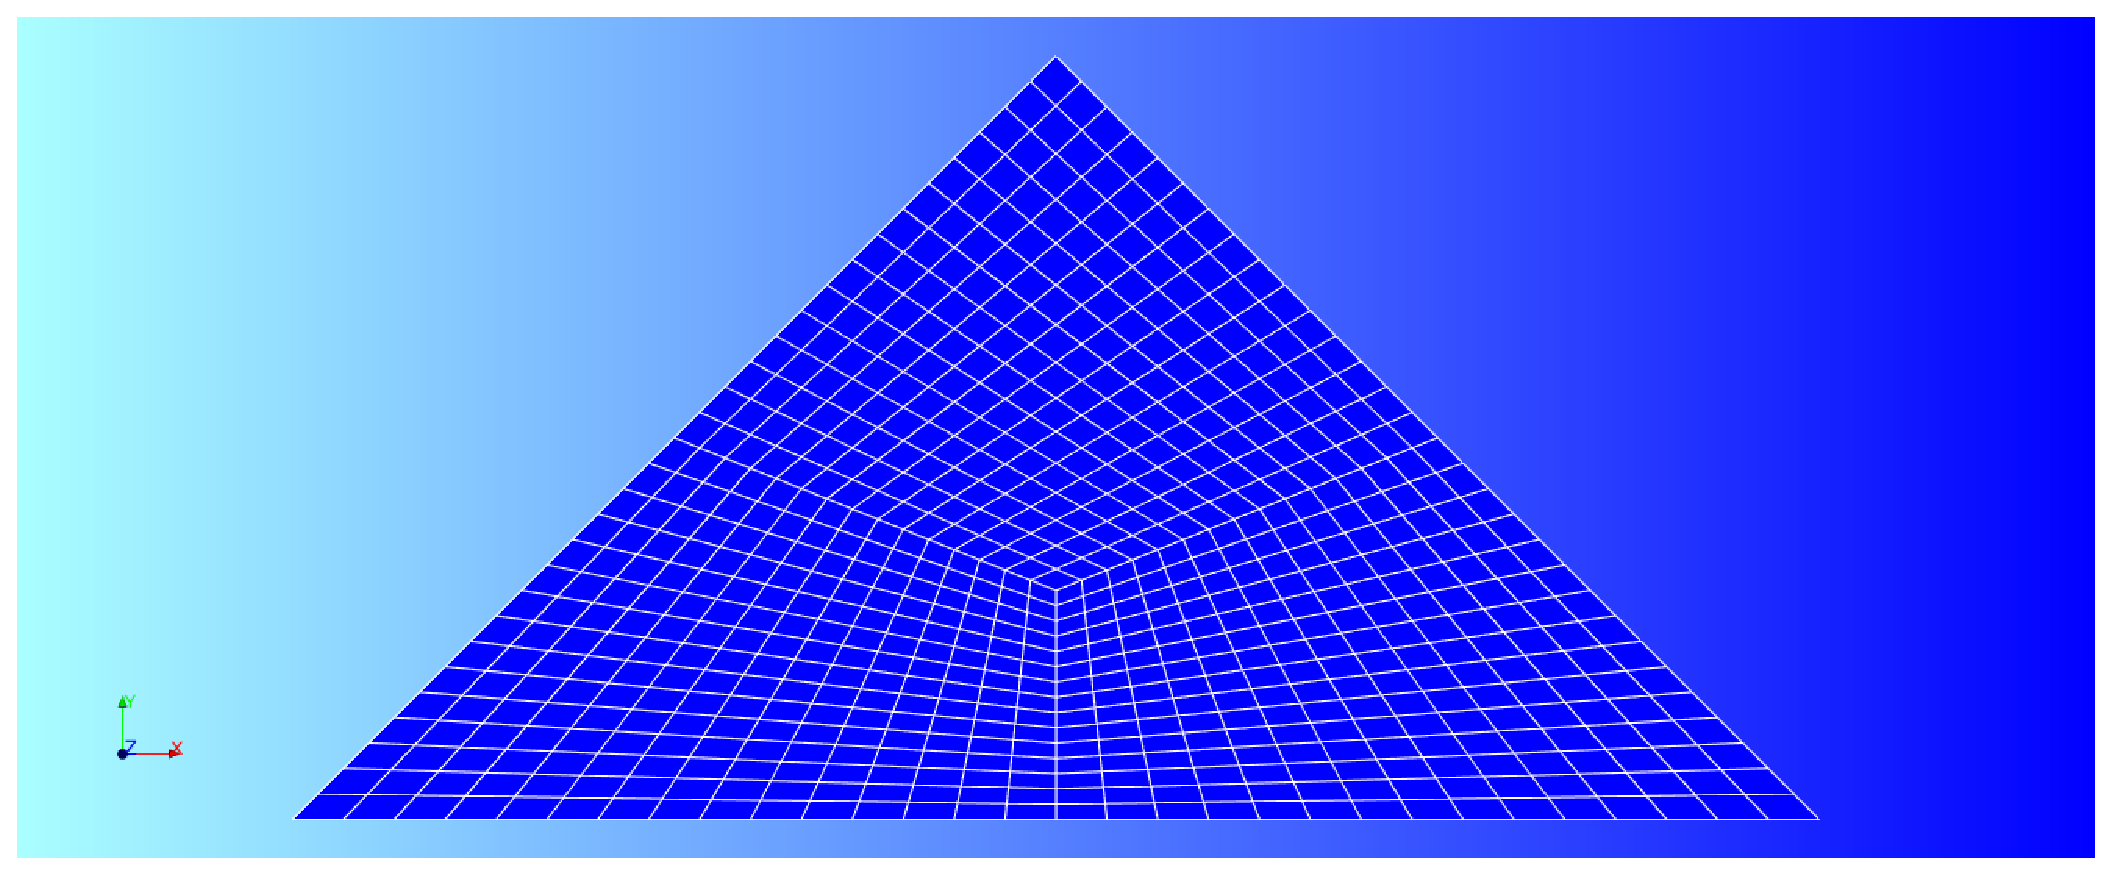
\includegraphics[width=1\linewidth]{Y_type_grid_example_1.eps}
	\end{figure}

\end{frame}

%SLIDE #?
\begin{frame}{Блочно -- структурированные сетки}

	\transdissolve[duration=0.1]
	\justifying
	\large

	\begin{center}
		\tikzstyle{root concept}+=[concept color=blue!80,minimum size=3.5cm]
		\tikz[mindmap]
			\node [concept] {Блочно -- структу-\\рированные сетки}
				child[concept color=yellow, grow=24, minimum size=3cm]
				{
					node[concept](root1) at (0,0) {Сетки с совмещением на внутренних границах}
				}
				child[concept color=green, grow=0, minimum size=3cm]
				{
					node[concept](root2) at (2,0) {Сетки без совмещений на внутренних границах}
				}
				child[concept color=red, grow=-24, minimum size=3cm]
				{
					node[concept](root2) at (0,0) {Компо-\\зитные сетки или химеры}
				};
	\end{center}

\end{frame}

%SLIDE #?
\begin{frame}{Блочно-структурированные сетки. H - O тип}

	\transdissolve[duration=0.1]
	\justifying
	\large

	\begin{figure}
		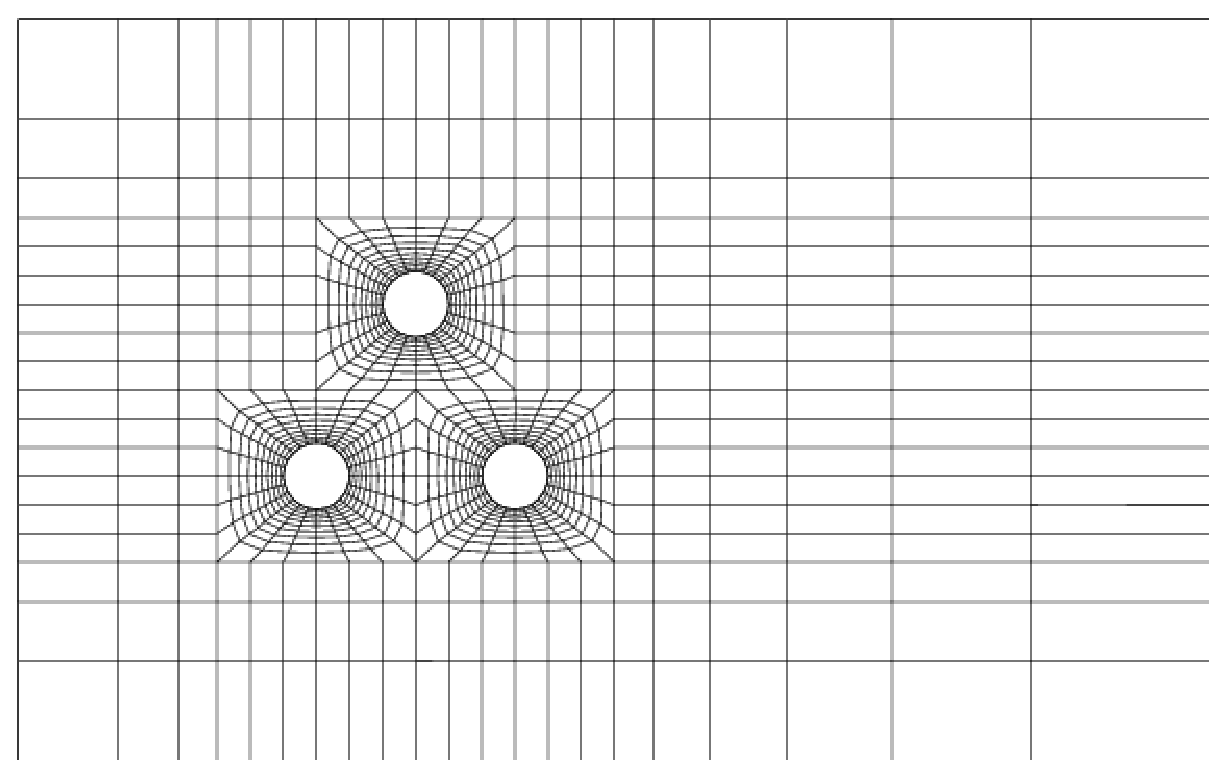
\includegraphics[width=0.7\linewidth]{O_H_type_grid_example_2.eps}
	\end{figure}

\end{frame}

%SLIDE #?
\begin{frame}{Блочно-структурированные сетки. H - O тип}

	\transdissolve[duration=0.1]
	\justifying
	\large

	\begin{figure}
		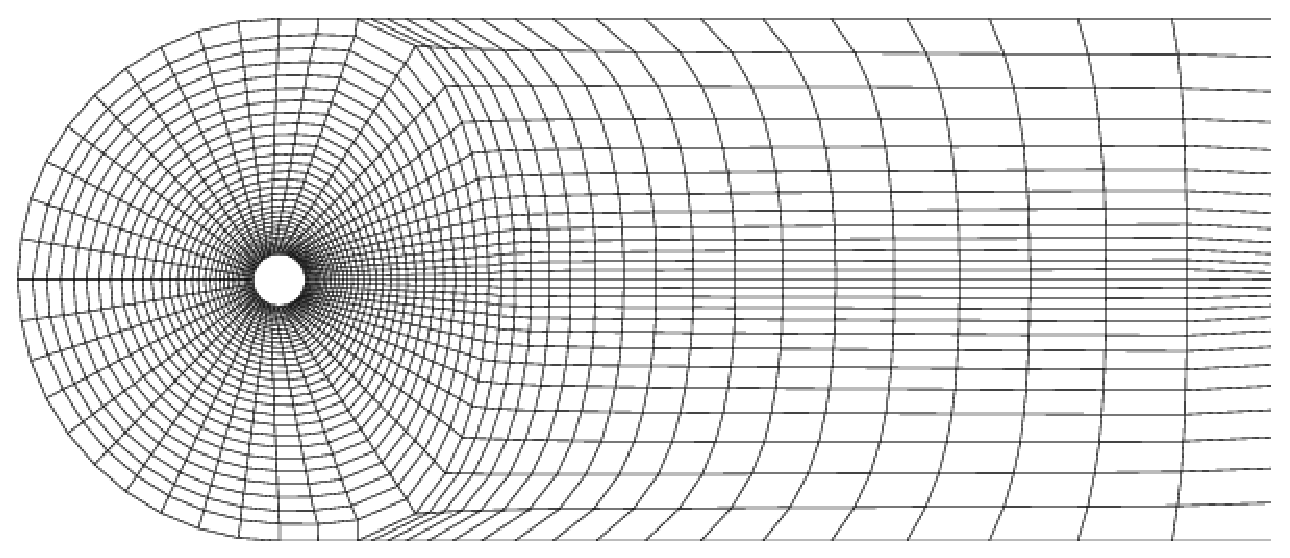
\includegraphics[width=0.8\linewidth]{O_H_type_grid_example_3.eps}
	\end{figure}

\end{frame}

%SLIDE #?
\begin{frame}{Композитные сетки}

	\transdissolve[duration=0.1]
	\justifying
	\large

	\begin{figure}
		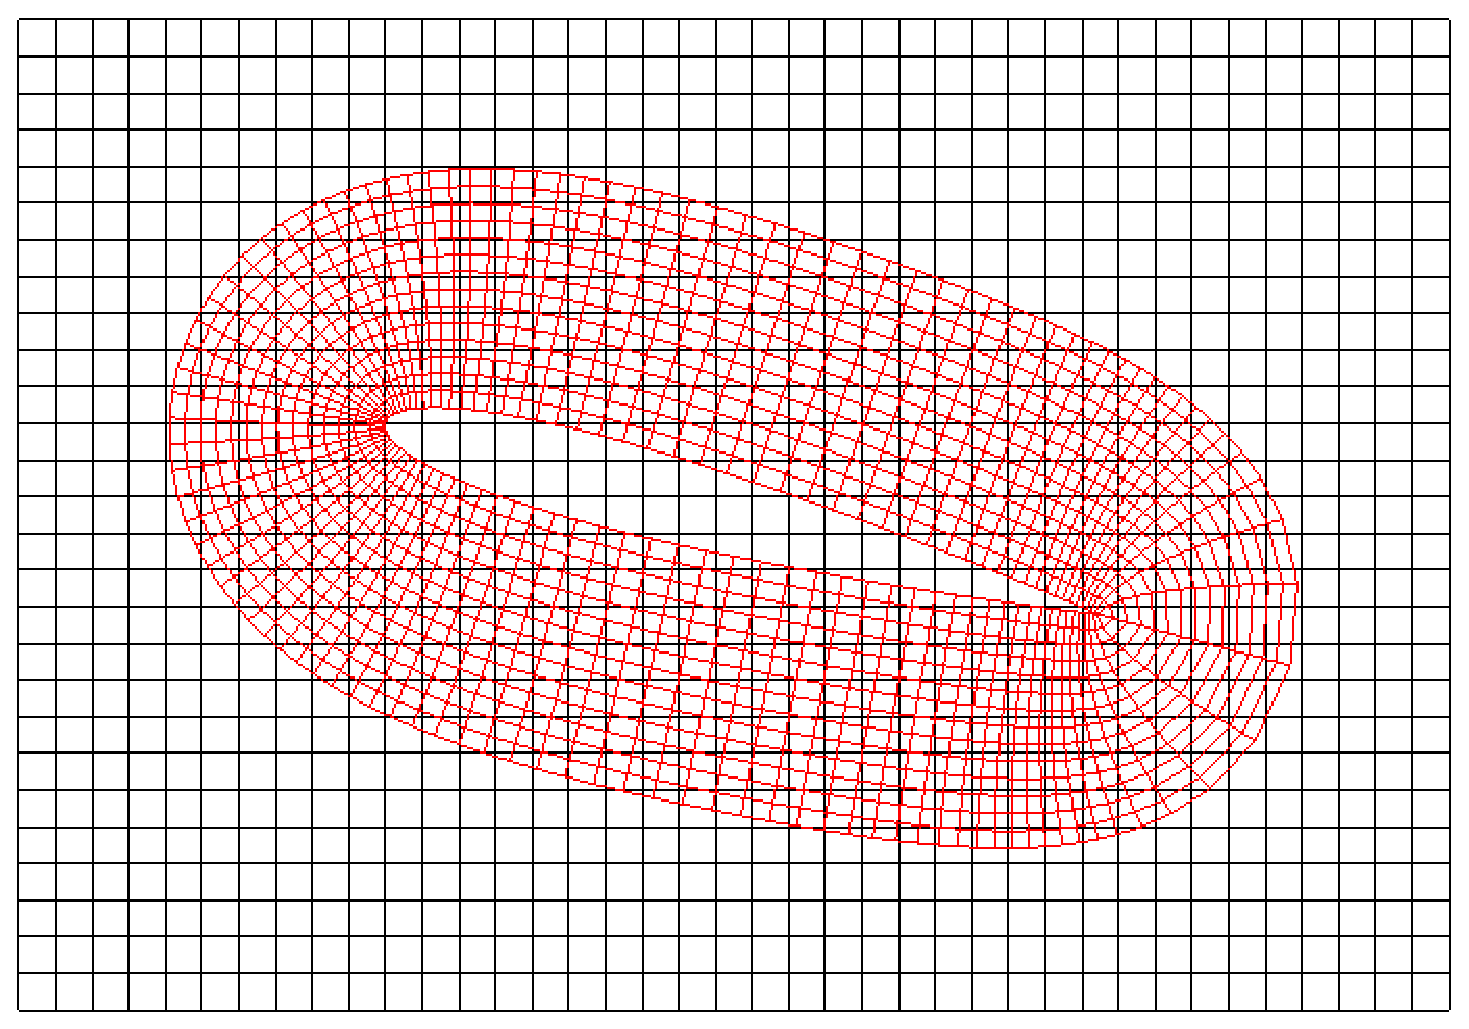
\includegraphics[width=0.6\linewidth]{overset_grid_example_1.eps}
	\end{figure}

\end{frame}

%SLIDE #?
\begin{frame}{Композитные сетки}

	\transdissolve[duration=0.1]
	\justifying
	\large
	
	Композитные сетки или химеры или погруженные сетки -- блочно - структурированные сетки с перекрывающимися блоками.\\
	\textbf{Достоинство}: можно использовать для двигающихся тел.\\
	\textbf{Недостаток}: на границах трудно соблюдать консервативноть численных методов.

\end{frame}

%SLIDE #?
\begin{frame}{Неструктурированные сетки}

	\transdissolve[duration=0.1]
	\justifying
	\large

	\begin{figure}
		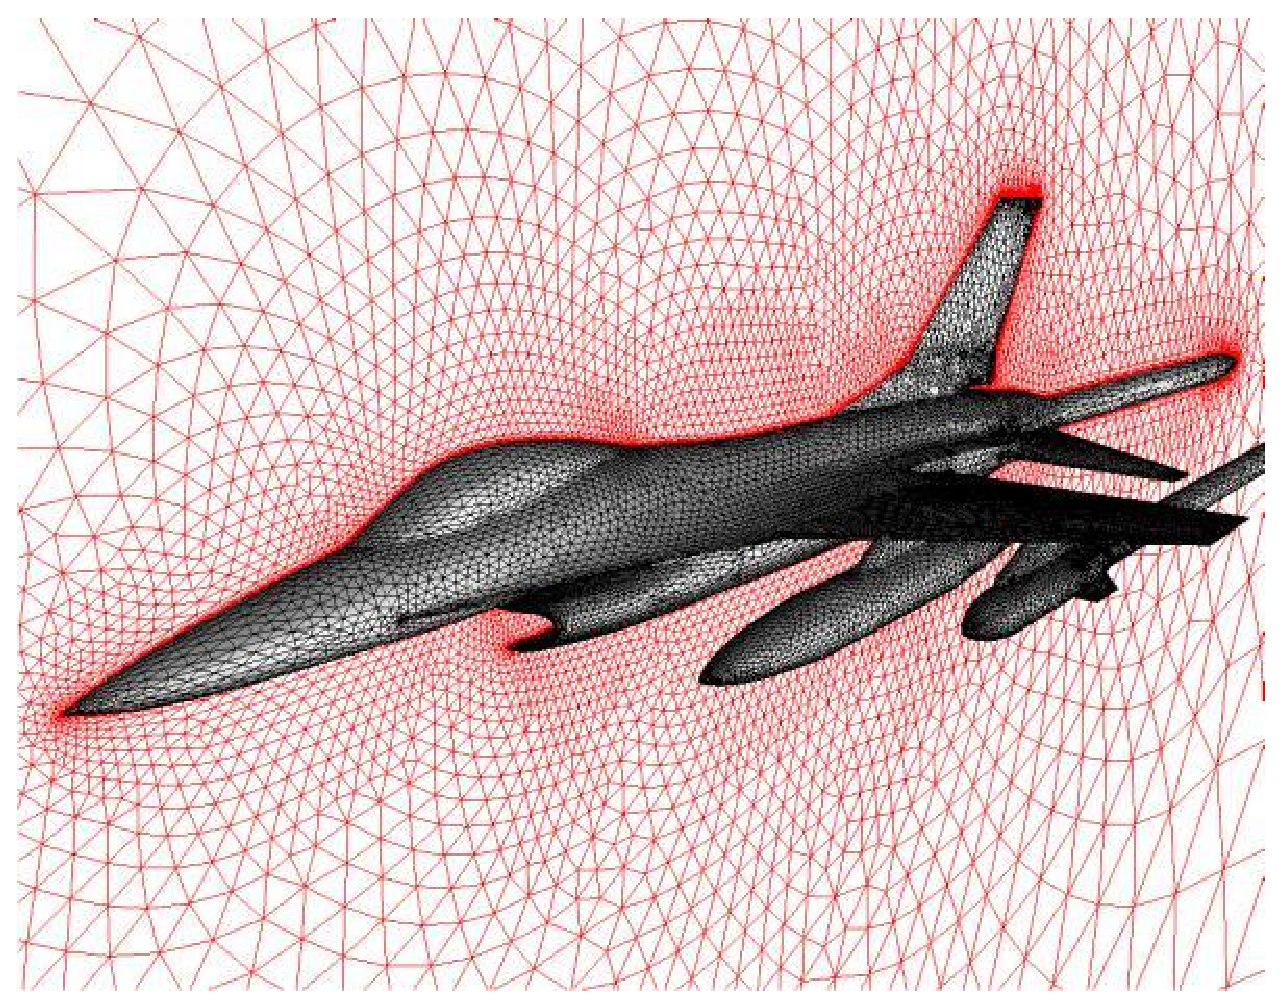
\includegraphics[width=0.6\linewidth]{unstructured_mesh_example_1.eps}
	\end{figure}

\end{frame}

%SLIDE #?
\begin{frame}{Достоинства и недостатки неструктурированных сеток}

	\transdissolve[duration=0.1]
	\justifying
	\large
	
	\begin{itemize}
		\item[+] Подходит для областей произвольных геометрий.
		\item[+] Нет ограничений на форму и количество соседних элементов.
		\item[+] Возможность локального измельчения.
		\item[-] Нерегулярность структуры данных, соответственно более
сложные и медленные алгоритмы решения.
	\end{itemize}

\end{frame}

%SLIDE #?
\begin{frame}{Сетка для моделирования подземной гидродинамики}

	\transdissolve[duration=0.1]
	\justifying
	\large

	\begin{figure}
		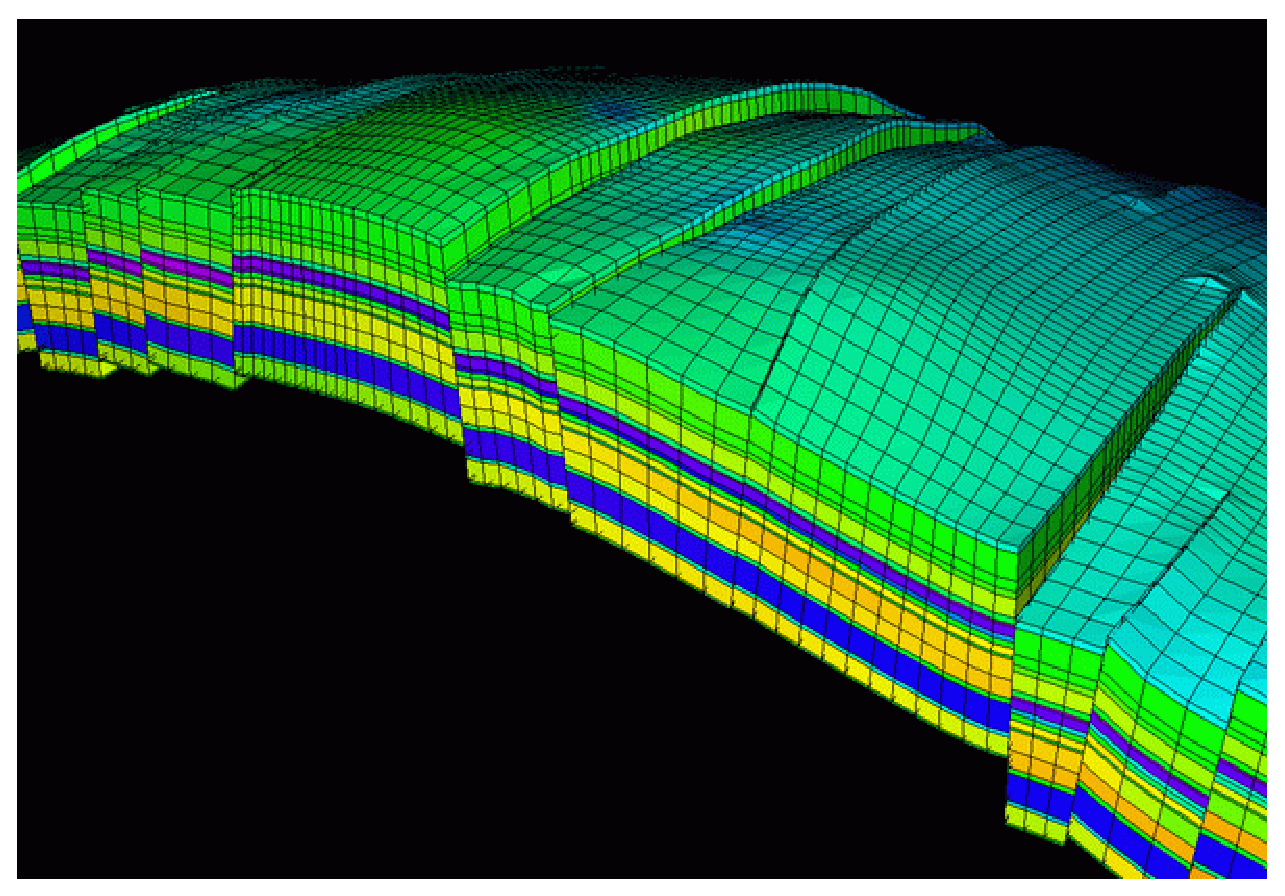
\includegraphics[width=0.65\linewidth]{oil_grid.eps}
	\end{figure}

\end{frame}

\end{document}